\documentclass[a4paper,11pt]{article}
% \pdfoutput=1 % if your are submitting a pdflatex (i.e. if you have
             % images in pdf, png or jpg format)
\usepackage{jcappub} % for details on the use of the package, please
                     % see the JCAP-author-manual
\usepackage[T1]{fontenc} % if needed
\usepackage{float} 
\usepackage{lmodern}
\usepackage{booktabs}
\usepackage{siunitx}
\usepackage[english]{babel}
\addto\captionsenglish{
  \renewcommand{\figurename}{Figure}
  \renewcommand{\tablename}{Table}
}
\usepackage[utf8]{inputenc}
\usepackage{natbib}
\usepackage[colorlinks=true, citecolor=blue, urlcolor=blue, linkcolor=blue]{hyperref} 
\usepackage{graphicx}
\usepackage{subfigure}% Include figure files
\usepackage[justification=raggedright]{caption}
\usepackage{tabularx}
\usepackage{dcolumn}% Align table columns on decimal point
\usepackage{bm}
% \usepackage{ulem}

\newcommand{\ms}{M_\odot}
\newcommand{\bmt}{{\bm{\theta}}}
\newcommand{\bmT}{{\bm{\Theta}}}
\newcommand{\bmH}{{\bm{H}}}
\newcommand{\rmd}{{\rm{d}}}

% \newcommand{\DL}[1]{\textcolor{red}{#1}} 
% \newcommand{\LS}[1]{\textcolor{cyan}{\bf #1}} 
% \newcommand{\YG}[1]{\textcolor{blue}{#1}} 
% \newcommand{\ZW}[2]{{\color{blue} \sout{#1} ZW: {#2}}} % For comment
% \newcommand{\Reply}[1]{{\bf\color{blue} #1}}

\title{Inference of Love-Q Relations with Gravitational Waves in Hierarchical Bayesian Framework}

%% %simple case: 2 authors, same institution
%% \author{A. Uthor}
%% \author{and A. Nother Author}
%% \affiliation{Institution,\\Address, Country}

% more complex case: 4 authors, 3 institutions, 2 footnotes
\author[a]{Zhihao Zheng,}

% The "\note" macro will give a warning: "Ignoring empty anchor..."
% you can safely ignore it.

\affiliation[a]{School of Yuanpei, Peking University,
Beijing 100871, China}
\affiliation[b]{Department of Astronomy, School of Physics, Peking University,
Beijing 100871, China}
\affiliation[c]{Kavli Institute for Astronomy and Astrophysics, Peking
University, Beijing 100871, China}
\affiliation[d]{Max Planck Institute for Gravitational Physics (Albert Einstein
Institute), Am M\"uhlenberg 1, D-14476 Potsdam-Golm, Germany}
\affiliation[e]{National Astronomical Observatories, Chinese Academy of
Sciences, Beijing 100012, China}

% \affiliation[a]{One University,\\some-street, Country}
% \affiliation[b]{Another University,\\different-address, Country}
% \affiliation[c]{A School for Advanced Studies,\\some-location, Country}

% e-mail addresses: one for each author, in the same order as the authors
\emailAdd{2300017794@stu.pku.edu.cn}

\abstract{Nuclear and gravity theories have predicted a universal relation between the tidal deformability $\Lambda$ 
and quadrupole moment $Q$ of neutron stars, offering a robust method for testing gravity. However, this Love-Q relation 
has not yet been directly measured through astrophysical observations. The detection of gravitational wave (GW) event GW170817 
provided a new channel for probing this relation, as both $\Lambda$ and $Q$ enter the GW waveform and can be inferred 
through parameter estimation. The next-generation GW detectors are expected to yield more GW observations with higher precision, 
enabling a measurement of the Love-Q relation. In this study, we construct a hierarchical Bayesian framework to conduct a systematic and 
efficient inference using simulated GW signals, aiming to determine the precision with which the Love-Q relation can be constrained. 
Our findings indicate that the results are dominated by the GW events with the highest signal-to-noise ratios and that a linear Love-Q model is sufficient for our dataset size. 
We also report a correlation in the posterior distribution of the parameters characterizing the Love-Q relation. 
Furthermore, our results suggest that dynamical Chern-Simons gravity can be constrained to $\xi_{\mathrm{CS}}^{1/4}<\mathcal{O}(10^2)$km, 
which is in agreement with the conclusion of previous studies.
}

\begin{document}
\maketitle
\flushbottom

%=============================
\section{Introduction}
\label{sec1}
%=============================

Neutron stars (NSs) serve as natural laboratories for testing nuclear and gravitational physics 
due to their extreme densities and strong gravitational fields---conditions unattainable in 
terrestrial and Solar System experiments. On the one hand, for nuclear physics, observations of NSs 
help us probe the equation of state (EOS) of high-density nuclear matter~\cite{Lattimer:2006xb}. 
For instance, the EOS can be constrained by the observed maximum NS mass~\cite{Hebeler:2013nza, Antoniadis:2013pzd} 
or the mass-radius relation~\cite{Lindblom:1992ApJ, Steiner:2010fz, Ozel:2010fw, Lackey:2014fwa, Pang:2021jta}. 
On the other hand, modified gravity theories predict variations in the interior structure of NSs
and their corresponding observable properties~\cite{Berti:2015itd, Shao:2022koz}. 
By measuring these properties, constraints can be placed on different gravity theories.

However, current observations do not have enough precision to determine the actual EOS. 
Consequently, attempts to test modified gravity theories are complicated by a degeneracy 
between the effects of modified gravity and the uncertainties in EOS~\cite{Yagi:2013bca, Silva:2020acr, Shao:2022koz}. 
To break this degeneracy, Yagi and Yunes~\cite{Yagi:2013bca, Yagi:2013awa} proposed using 
universal relations among NS properties, including the moment of inertia ($I$), 
tidal Love number (or tidal deformability $\Lambda$), and the dimensionless spin-induced quadrupole moment ($Q$). 
These I-Love-Q relations are EOS-insensitive (with variation of about $1\%$ or less) yet they can be dependent on 
the underlying gravity theory. Hence, by independently measuring any two of the I-Love-Q trio, 
one can test gravity theories avoiding the degeneracy with the uncertainties from nuclear physics.

The recent observation of GW170817 demonstrated that gravitational waves (GWs) emitted during binary neutron star (BNS) 
coalescences have opened up a new observational window for investigating NS properties~\cite{LIGOScientific:2017vwq, LIGOScientific:2018cki, LIGOScientific:2018hze}. 
In a BNS system, tidal deformation occurs to each star due to the gravitational field of its companion~\cite{Hinderer:2007mb, Damour:2009vw}. 
This interaction influences the inspiral of the binary, thereby leaving a distinct signature on the emitted GWs~\cite{Vines:2011ud, Favata:2013rwa, Wade:2014vqa, Baiotti:2019sew, Chatziioannou:2020pqz}.
The effect is characterized by the tidal deformability $\Lambda=2k_2/(3C^5)$, 
where $k_2$ is the tidal Love number and $C$ is the NS compactness~\cite{Flanagan:2007ix}. Besides, a rotating NS experiences another deformation due to its 
spin, which induces a quadrupole moment $\mathcal{Q}=-Q\chi^2 m^3$ (spin-induced quadrupole moment, SIQM), where $Q$ is the dimensionless quadrupole moment,
\footnote{We only talk about the dimensionless quadrupole moment later in the text and for simplicity, we ref $Q$ as quadrupole moment without causing ambiguity.} 
$\chi$ is the NS dimensionless spin and $m$ is the NS mass~\cite{Hartle:1968, Laarakkers:1997hb}. Similar to tidal deformability, the quadrupole moment also enters the 
GW waveform~\cite{Poisson:1997ha, Harry:2018hke, Samajdar:2019ulq, Abac:2023ujg} and is therefore a key parameter to probe the properties of compact binaries with GW signals~\cite{Agathos:2015uaa, Krishnendu:2017shb, Krishnendu:2019tjp, Lyu:2023zxv}. 

Future next-generation ground-based GW detectors, including the Cosmic Explorer (CE)~\cite{Reitze:2019iox, Reitze:2019dyk} and the Einstein Telescope (ET)~\cite{Punturo:2010zz, Hild:2010id, Sathyaprakash:2012jk}, 
will detect much more GW signals (up to about $10^5$--$10^6$ events per year)~\cite{LIGOScientific:2017zlf, Sathyaprakash:2019yqt, Kalogera:2021bya, Samajdar:2021egv} 
and more precise measurements of the tidal deformability and the quadrupole moment~\cite{Yagi:2013awa, Samajdar:2020xrd}, thanks to their increased sensitivity and lower cutoff frequencies. 
With more high-precision GW data, one can combine the measurements of $\Lambda$ and $Q$ to infer the Love-Q relation from GW observations. 
While Samajdar and Dietrich~\cite{Samajdar:2020xrd} have performed a preliminary analysis concluding that the next-generation GW detectors 
will allow for a measurement of this relation, a more systematic and efficient framework is needed to join a considerable number of GW events and provide a robust estimation of the Love-Q relation. 

Hierarchical Bayesian inference presents an appropriate method for this problem and has been applied in population analyses and EOS constraints~\cite{Mandel:2009nx, Mandel:2009pc, Adams:2012qw, Lackey:2014fwa, Mandel:2018mve, Thrane_2019, KAGRA:2021duu, Wang:2024xon}.
In our case, the Love-Q relation parameters can be regarded as the hyper parameters, and in hierarchical Bayesian framework, 
the inference of these hyper parameters is separated from the inference of the GW waveform parameters to achieve a higher level of computational efficiency. 

In this work, we construct such a hierarchical Bayesian framework to infer the Love-Q relation from simulated GW signals, exploring its potential for combining future GW observations with next-generation detectors. 
We also investigate how the results are impacted by the number of GW events analysed and by the specific parameterization of Love-Q relation. 
Furthermore, as a direct application of our results, we discuss how the inferred Love-Q relation can be used to place constraints on dynamical Chern-Simons gravity.

This paper is organized as follows. In section~\ref{sec2} we construct the hierarchical Bayesian framework and derive the posterior of the hyper parameters. 
The simulation procedure is explained in detail in section~\ref{sec3}. Then we present the results of our inference and discuss the inpact from different Love-Q relation parameterizations in section~\ref{sec4}. 
We compare our inference results with the predictions of the dynamical Chern-Simons gravity as a test in section~\ref{sec5}. Finally, we conclude this work in section~\ref{sec6}.


%=============================
\section{Hierarchical Bayesian Inference of Love-Q Relation Parameters}
\label{sec2}
%=============================

%=============================
\subsection{Preliminary} 
\label{sec2_1}
%=============================
In our simulation, we parameterize the Love-Q relation in linear (2-d) and quartic polynomial (5-d) 
manners as follows
\begin{subequations}
\label{Love-Q Relation}
\begin{equation}
\label{5-d_Love_Q_eq}
    \ln Q_{5d}=a_5 + b_5 \ln \Lambda + c_5 \ln^2\Lambda + d_5 \ln^3\Lambda + e_5 \ln^4 \Lambda\,,
\end{equation}
\begin{equation}
\label{2-d_Love_Q_eq}
    \ln Q_{2d} = a_2 + b_2 \ln \Lambda\,.
\end{equation}
\end{subequations}
For the Yagi-Yunes relation, we have $a_5=0.1940$, $b_5=0.09163$, $c_5=0.04812$, 
$d_5=-4.283\times10^{-3}$, and $e_5=1.245\times10^{-4}$~\cite{Yagi_2017}. In figure~\ref{relative_difference}, 
we plot the Yagi-Yunes relation as well as its linear fit and in this case, the relative difference in $\ln Q$ 
between these two parameterization manners is within $\mathcal{O}(1) \%$. No matter how we parameterize the 
Love-Q relation, these fitting coefficients do not enter the GW waveform and therefore cannot be directly 
measured from GW signals. Instead, different combinations of fitting coefficients determine different Love-Q relations, 
leading to an impact on the GW signals. In other words, such a Love-Q relation provides a delta-function-type 
prior for GW parameters $\Lambda_i$ and $Q_i$. Correspondingly, the fitting coefficients of our Love-Q relation 
can be regarded as hyper parameters, denoted as $\bm{H}$. Then we write down the conditional prior
\begin{equation}
\label{delta function prior}
\pi(Q_i|\Lambda_i,\bm{H}) = \delta(Q_i-f(\Lambda_i;\bm{H}))\,.
\end{equation}

\begin{figure}[tbp]
\centering
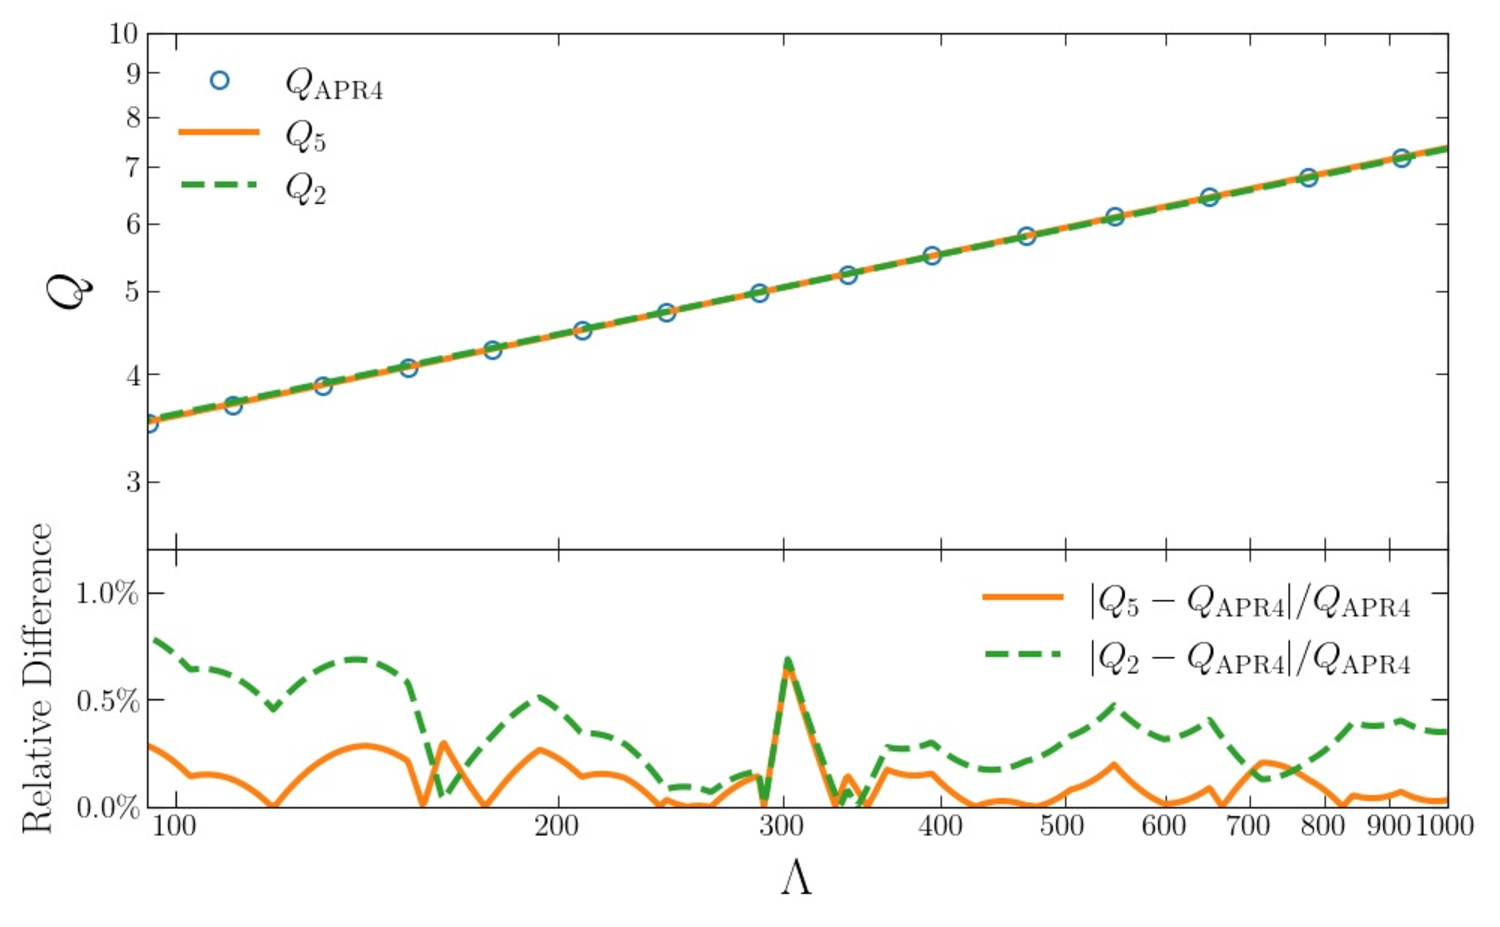
\includegraphics[width=0.8\textwidth]{2d-5d difference.pdf}% Here is how to import EPS art
\caption{\label{relative_difference} The upper panel shows the relation between $\ln \Lambda$ and $\ln Q$ 
for the Yagi-Yunes relation (5-d) and its linear fit (2-d). The lower panel shows the relative difference 
of 5-d and 2-d results.}
\end{figure}

%=============================
\subsection{Derivation}
\label{sec2_2}
%=============================

Hierarchical Bayesian inference is a framework that allows us to go beyond single GW events, joining a set 
of single events together to probe the Love-Q relation. In this framework, our main objective is to derive 
the posterior density function (PDF) $p(\bm{H}|D)$ for the fitting coefficients of the Love-Q relation, 
i.e. the hyper parameters. The data $D=\{\bm{d}_1,...,\bm{d}_n\}$ contains data streams $\bm{d}_i$ of $n$ 
GW events from the detector network. Note that we make no assumptions of EOS in the hierarchical Bayesian 
inference part and EOS does not emerge in the conditional probability functions, given that the Love-Q relation 
is EOS-insensitive. To acquire the marginalized posterior for only hyper parameters, we marginalize over the entire parameter space
\begin{equation}
\label{bayes1}
p(\bm{H}|D) = \int p(\bm{H},\bm{\theta}_1,...,\bm{\theta}_n|D) \text{d}\bm{\theta}_1...\text{d}\bm{\theta}_n\,.
\end{equation}
Then applying Bayes' theorem
\begin{equation}
\label{bayes2}
p(\bm{H},\bm{\theta}_1,...,\bm{\theta}_n|D)=\pi(\bm{H},\bm{\theta}_1,...,\bm{\theta}_n)\frac{p(D|\bm{H},\bm{\theta}_1,...,\bm{\theta}_n)}{p(D)}\,,
\end{equation}
where $\pi(\bm{H},\bm{\theta}_1,...,\bm{\theta}_n)$ is the prior probability density for the fitting coefficients 
and waveform parameters, $p(D|\bm{H},\bm{\theta}_1,...,\bm{\theta}_n)$ is the likelihood function, and $p(D)$ is 
the evidence which we do not need to calculate. Then we derive the prior and likelihood as follows.

\paragraph{Prior}
Considering the fact that the $n$ events are independent, the prior can be decomposed into parts of hyper parameters 
and waveform parameters using the product rule of probability $p(A,B)=p(A)p(B|A)$
\begin{equation}
\label{bayes3}
\pi(\bm{H},\bm{\theta}_1,...,\bm{\theta}_n) = \pi(\bm{H}) \prod_{i=1}^n \pi(\bm{\theta}_i|\bm{H})\,.
\end{equation}
We divide the set of waveform parameters for each event $\bm{\theta}_i$ into three categories: the tidal deformability 
parameters $\bm{\Lambda}_i=\{\Lambda_{1i},\Lambda_{2i}\}$, the quadrupole moment parameters $\bm{Q}_i=\{Q_{1i},Q_{2i}\}$, 
and the nuisance parameters $\bm{\xi}_i$. Since no particular EOS is chosen here, the $m-\Lambda$ relation remains undetermined. 
Therefore, we assume that the prior distributions for nuisance parameters, including the two mass parameters, 
are independent of $\bm{\Lambda}_i, \bm{Q}_i$ and $\bm{H}$. In this way, the conditional prior for the waveform parameters 
in eq.~(\ref{bayes3}) can be further decomposed with the product rule
\begin{equation}
\label{prior}
\pi(\bm{\theta}_i|\bm{H})=\pi(\bm{\Lambda}_i|\bm{H})\pi(\bm{Q}_i|\bm{\Lambda}_i,\bm{H})\times\pi(\bm{\xi}_i)\,.
\end{equation}

\paragraph{Likelihood}
Analogously, we decompose the likelihood into a product of single-event likelihoods for $n$ independent BNS observations
\begin{subequations}
\begin{align}
p(D|\bm{H},\bm{\theta}_1,...,\bm{\theta}_n)&=\prod_{i=1}^{n}p(\bm{d}_i|\bm{H},\bm{\theta}_i)\\
&=\prod_{i=1}^{n}p(\bm{d}_i|\bm{\theta}_i)\,.
\end{align}   
\end{subequations}
Note that in the second line we have used the fact that the hyper parameters do not enter the waveform thus the likelihood 
only depends on $\bm{\theta}_i$, i.e. $p(\bm{d}_i|\bm{H},\bm{\theta}_i)=p(\bm{d}_i|\bm{\theta}_i)$.


Based on the derivation above, now the marginalized PDF (eq.~(\ref{bayes1})) is
\begin{equation}
\label{hierarchical bayes}
\begin{aligned}
p(\bm{H}|D)&=\frac{1}{p(D)}\pi(\bm{H})\int \text{d}\bm{\theta}_1...\text{d}\bm{\theta}_n \prod_{i=1}^n \left[\pi(\bm{\Lambda}_i|\bm{H})\pi(\bm{Q}_i|\bm{\Lambda}_i,\bm{H})\pi(\bm{\xi}_i)p(\bm{d}_i|\bm{\theta}_i)\right] \\
&=\frac{1}{p(D)} \pi(\bm{H}) \prod_{i=1}^n
\int \text{d}\bm{\Lambda}_i\text{d}\bm{Q}_i\pi(\bm{\Lambda}_i|\bm{H})\delta\left(\bm{Q}_i-\bm{f}(\bm{\Lambda}_i;\bm{H})\right) \int \text{d}\bm{\xi}_i \pi(\bm{\xi}_i)p(\bm{d}_i|\bm{\theta}_i)\\
&=\frac{1}{p(D)} \pi(\bm{H}) \prod_{i=1}^n
\int \text{d}\bm{\Lambda}_i\pi(\bm{\Lambda}_i|\bm{H})L_i\left(\bm{\Lambda}_i,\bm{f}(\bm{\Lambda}_i;\bm{H})\right)\,.
\end{aligned}
\end{equation}
where we define the quasi-likelihood function for $\bm{\Lambda}_i,\bm{Q}_i$ as
\begin{equation}
\label{quasi-likelihood}
    L_i(\bm{\Lambda}_i,\bm{Q}_i)=\int \text{d}\bm{\xi}_i \pi(\bm{\xi}_i)p(\bm{d}_i|\bm{\theta}_i)\,.
\end{equation}

What we need to compute now are the quasi-likelihood functions (eq.~(\ref{quasi-likelihood})) for each GW event and then 
substitute them into eqs.~(\ref{hierarchical bayes}). In hierarchical Bayesian inference, these quasi-likelihood functions 
can be calculated in advance to reduce computational cost, considering that the hyper parameters $\bm{H}$ do not appear 
in eq.~(\ref{quasi-likelihood})~\cite{Lackey:2014fwa, Thrane:2018qnx, Golomb:2021tll}. We start from Bayes' theorem for 
the $i\text{-th}$ GW event
\begin{equation}
\label{single bayes}
    p(\bm{\theta}_i|\bm{d}_i)\propto \pi(\bm{\theta}_i|\varnothing)p(\bm{d}_i|\bm{\theta}_i)\,,
\end{equation}
where $\pi(\bm{\theta}_i|\varnothing)$ is the default prior chosen as long as it is sufficiently uninformative\cite{Thrane:2018qnx}, 
and $p(\bm{d}_i|\bm{\theta}_i)$ is the single-event likelihood~\cite{Finn:1992wt},
\begin{equation}
p(\bm{d}_i|\bm{\theta}_i)\propto \mathrm{e}^{-\frac{1}{2}\langle d_i-h(\bm{\theta}_i),d_i-h(\bm{\theta}_i)\rangle}\,.
\end{equation}
$h(\bm{\theta}_i)$ is given by the waveform model in section~\ref{sec2_1} while $\langle g, h\rangle$ is the inner product 
of $g(t)$ and $h(t)$ weighted by the power spectrum density(PSD) of $S_n(f)$ of the noise.
\begin{equation}
    \langle g, h\rangle:=2\text{Re}\int_{-\infty}^{\infty}\frac{\tilde{g}^{*}(f)\tilde{h}(f)}{S_n(|f|)} \text{d}f\,,
\end{equation}
where $\tilde{g}(f)$ and $\tilde{h}(f)$ are the Fourier transforms of $g(t)$ and $h(t)$.

What we choose for the default prior in eq.~(\ref{single bayes}) is not so important as long as it is sufficiently 
uninformative~\cite{Thrane:2018qnx}. Rearranging terms of eq.~(\ref{single bayes}) and substituting it into 
eq.~(\ref{quasi-likelihood}), we obtain
\begin{equation}
\label{quasi-posterior}
\begin{aligned}
    L_i(\bm{\Lambda}_i,\bm{Q}_i) &= \int \text{d}\bm{\xi}_i \pi(\bm{\xi}_i)p(\bm{d}_i|\bm{\theta}_i) \\
    &\propto \int \text{d}\bm{\xi}_i \frac{\pi(\bm{\xi}_i)}{\pi(\bm{\theta}_i|\varnothing)}p(\bm{\theta}_i|\bm{d}_i)\,,
\end{aligned}  
\end{equation}
which allows us to construct the quasi-likelihood function with posteriors of each event. In particular, as long as 
we choose flat priors for tidal and quadrupole moment parameters, the quasi-likelihood function is proportional to 
the marginalized posterior for every single event.


%=============================
\section{Simulation}
\label{sec3}
%=============================

%=============================
\subsection{Waveform, Population and Detectors}
\label{sec3_1}
%=============================

For our simulation, we adopt the {\sc imrphenomxas\_nrtidalv3} waveform model~\cite{Abac:2023ujg}, 
which is an aligned spin waveform and includes tidal amplitude corrections as well as spin-induced quadrupole moment terms up to 3.5PN. 
The parameter set is composed of the binary masses $m_1$ and $m_2$, the dimensionless tidal deformabilities $\Lambda_i$ 
and spin-induced quadrupole moments $Q_i$ of each component, the dimensionless spin aligned with the direction of the 
orbital angular momentum $\chi_i$, the luminosity distance to the source $D_L$, the merge time $t_c$, the right ascension 
$\alpha$ and declination $\delta$, the inclination angle $\iota$, the GW polarization angle $\psi$ and the phase of 
coalescence $\phi_c$. We denote the entire parameter set as a vector $\bm{\theta}$, i.e.
\begin{equation}
\label{parameter set}
\bm{\theta} = \{m_1,m_2,\Lambda_1,\Lambda_2,Q_1,Q_2,\chi_1,\chi_2,D_L,t_c,\alpha,\delta,\iota,\psi,\phi_c\}\,.
\end{equation}
Since our curiosity lies in tidal deformability and quadrupole moment, other parameters are regarded as nuisance parameters, 
which are denoted as $\bm{\xi}$.

We adopt the BNS mass population model proposed by Farrow~et~al.~\cite{Farrow:2019xnc}, in which the two BNS components do not necessarily 
have the same mass distribution. According to their spin magnitude, the model divides BNS into a recycled star and a nonrecycled 
(\emph{slow}) one, for which the masses are labeled $m_r$ and $m_s$, respectively. The distribution of $m_r$ has two Gaussian 
components while $m_s$ follow a Uniform distribution,
\begin{subequations}
\label{mass population}
\begin{equation}
    P(m_r) = \alpha \mathcal{N}(\mu_1, \sigma_1) + (1-\alpha) \mathcal{N}(\mu_2, \sigma_2)\,,
\end{equation}
\begin{equation}
    P(m_s) = \mathcal{U}(m_s^l, m_s^u)\,,
\end{equation}
\end{subequations}
where $\alpha=0.68$, $\mu_1=1.34M_{\odot}$, $\sigma_1=0.02M_{\odot}$, $\mu_2=1.47M_{\odot}$, $\sigma_2=0.15M_{\odot}$ and $m_s^l=1.14M_{\odot}$, $m_s^u=1.46M_{\odot}$. When generating simulation GW signals, for each event we just select the larger one of $m_r$ and $m_s$ as the primary mass $m_1$ and the other as the secondary mass $m_2$, since we always demand $m_1 \geq m_2$.

The tidal deformability and quadrupole moments of the binary are calculated from the stellar mass, assuming the AP4 EOS, 
which is a soft EOS consistent with the LIGO-Virgo tidal measurements~\cite{LIGOScientific:2017vwq, LIGOScientific:2018cki, LIGOScientific:2018hze}. 
Refs.~\cite{Yagi:2013awa, Atta:2024ckt} demonstrates in detail how to derive tidal deformability $\Lambda_i$ and quadrupole moment $Q_i$ 
given the mass $m_i$ and the EOS. For the dimensionless spin component $\chi_r$ of recycled stars, we adopt a uniform distribution $\mathcal{U}(-0.5,0.5)$, 
while in the case of slow stars, the spin $\chi_s$ is drawn from $\mathcal{U}(-0.1,0.1)$.

Using the cosmological parameters provided by the Planck Collaboration~\cite{Planck:2018vyg}, we simulate 1000 GW sources distributed 
uniformly in co-moving volume from 15Mpc to 150Mpc~\cite{Fishbach:2018edt, KAGRA:2021duu}, with isotropic sky locations and orientations. This corresponds to the observed local 
merger rate $R=320_{-270}^{+490}\,\mathrm{Gpc}^{-3}\mathrm{yr}^{-1}$ from current GW detections~\cite{LIGOScientific:2020aai}. 
To reduce the calculation cost, we only select sources with the highest signal-to-noise ratio (SNR) for Bayesian inference. 
Without loss of generality, all these GW events are injected with an arbitrary coalescence time $t_c=0$.

A ground-based network consisting of two CE detectors and one ET detector is selected as the GW detectors. 
We simulate data in noise generated with designed sensitivity curves taken as CE-2~\cite{Reitze:2019iox, Reitze:2019dyk} and ET-D~\cite{Punturo:2010zz, Hild:2010id, Sathyaprakash:2012jk}. 
The two CE detectors are positioned at the current sites of the two LIGO detectors, while the ET detector is set at the current location of the 
Virgo detector with a triangular shape. For these next-generation detectors, their lower cutoff frequencies $f_{\text{low}}$ can reach about 1 Hz. 
Compared to $f_{\text{low}}=28$ Hz for advanced LIGO and Virgo, a smaller $f_{\text{low}}$ means an improvement in both the signal-to-noise ratio and the duration 
when the signal is visible in band.

%=============================
\subsection{Implementation}
\label{sec3_2}
%=============================

The evaluation of the marginalized posterior for hyper parameters can be divided into two steps, similar to 
Refs.~\cite{Steiner:2010fz, Lackey:2014fwa, Wang:2024xon}. We first perform Bayesian inference for each event using some sampling methods, 
such as the Markov Chain Monte Carlo (MCMC) method~\cite{Christensen:1998gf, Christensen:2004jm} and nested sampling~\cite{Skilling:2004pqw, Skilling:2006gxv}, 
generating posterior samples to acquire the quasi-likelihood (eq.~(\ref{quasi-posterior})) through density estimation; 
then we substitute the quasi-likelihoods into eq.~(\ref{hierarchical bayes}) to obtain the posterior of hyper parameters. 

In the first step, when conducting single-event Bayesian inference, we choose $\mathcal{M}$ and $\eta$ as mass parameters. 
In this way, the parameter set of single-event Bayesian inference becomes $\bm{\theta} = \{\mathcal{M},\eta,\Lambda_1,\Lambda_2,Q_1,Q_2,\chi_1,\chi_2,D_L,t_c,\alpha,\delta,\iota,\psi,\phi_c\}$. 
The priors of $\mathcal{M},\eta,\chi_1,\chi_2,t_c,\phi_c$ are uniform, while the prior of $D_L$ is uniform in the co-moving volume and source frame time. 
Isotropy is ensured by setting priors for the angle variables $\alpha,\delta,\iota,\psi$. For tidal and quadrupole moment parameters, we treat $\Lambda_s$ and $Q_s$ 
of the slow binary component as nuisance parameters, considering that the spin-induced quadrupole moment is poorly estimated with low spin~\cite{Yagi:2013awa}. 
And we select uniform priors for $\Lambda_1,\Lambda_2$ and $Q_1,Q_2$ so that eq.~(\ref{quasi-posterior}) can be further simplified as
\begin{equation}
    \label{quasi-marginalized}
    \begin{aligned}
        L_i(\Lambda_{ri},Q_{ri}) &\propto \int \text{d}\bm{\xi}_i \frac{\pi(\bm{\xi}_i)}{\pi(\bm{\theta}_i|\varnothing)}p(\bm{\theta}_i|\bm{d}_i) \\
        &\propto \int \text{d}\bm{\xi}_i p(\bm{\theta}_i|\bm{d}_i) \\
        &\propto p(\Lambda_{ri},Q_{ri}|\bm{d}_i)\,,
    \end{aligned}  
\end{equation}
where $\Lambda_{ri}$ and $Q_{ri}$ are the tidal deformability and quadrupole moment of the recycled 
binary component of the $i$th event, respectively. Eq.~(\ref{quasi-marginalized}) indicates that the quasi-
likelihood is proportional to the marginalized posterior, revealing that we can directly construct the quasi-
likelihood from posterior samples.

After sampling, we obtain the quasi-likelihood of each event from $\Lambda_r$ and $Q_r$ samples. To complete the integral in eq.~(\ref{hierarchical bayes}), 
we must create a functional form for each quasi-likelihood using the posterior samples. Following Golomb and Talbot~\cite{Golomb:2021tll}, 
we introduce the Gaussian mixture model (GMM) method developed by Ref.~\cite{Talbot:2020oeu} as the density estimation method to obtain the quasi-likelihood with eq.~(\ref{quasi-likelihood}). 
Substitute the results of density estimation into eq.~(\ref{hierarchical bayes}), and then the likelihood function of the hyper parameter estimation can be constructed.

In the second step, we sample the integrand of eq.~(\ref{hierarchical bayes}) with Bayesian inference. For hyper parameters $\pi(\bm{H})$, 
we use uniform priors with the boundaries listed in Table~\ref{prior_table} and for the prior $\pi(\bm{\Lambda}_i|\bm{H})$, 
we use the uniform distribution $\mathcal{U}(10,2000)$. For Bayesian inference in both steps, posterior samples are generated with {\sc NESSAI}~\cite{michael_j_williams_2025_14627250, PhysRevD.103.103006, Williams:2023ppp} 
of the {\sc BILBY}~\cite{Ashton:2018jfp} package. 20 simulated GW sources with the highest SNRs and spins are selected from 1000 sources, 
which are generated as described in section~\ref{sec3_1}.

\begin{table}[htbp]
    \centering
    \sisetup{
        table-align-text-post = false, 
        separate-uncertainty = true 
    }
    \caption{\label{prior_table}The best fit values of Yagi-Yunes relation and the priors of the hyper parameters in linear and 
    quartic polynomial fitting models for the Bayesian inference.}
    \begin{tabular}{
        l
        S[table-format=-1.4]
        S[table-format=1.5]
        S[table-format=1.3e-1]
        S[table-format=-1.3e-1]
        S[table-format=1.3e-1]
    }
        \toprule
        \multicolumn{6}{c}{Best fit values} \\
        %\cmidrule(l){2-6}
        Parameter & {$a_i$} & {$b_i$} & {$c_i$} & {$d_i$} & {$e_i$} \\
        \midrule

        5-d &  0.1940 & 0.0916 & 4.812e-2 & -4.283e-3 & 1.245e-4 \\
        4-d &  0.1290 & 0.1480  & 3.021e-2 & -1.817e-3 & {/}      \\
        3-d & -0.0709 & 0.2775  & 3.220e-3 & {/}       & {/}      \\
        2-d & -0.1457 & 0.3094  & {/}      & {/}       & {/}      \\
        
        \midrule

        \multicolumn{6}{c}{Prior} \\
        %\cmidrule(l){2-6}
        Parameter & {$a_i$} & {$b_i$} & {$c_i$} & {$d_i$} & {$e_i$} \\
        \midrule

        5-d & {$\mathcal{U}(-5.0, 5.0)$} & {$\mathcal{U}(-1.0, 1.0)$} & {$\mathcal{U}(-0.5, 0.5)$} & {$\mathcal{U}(-0.1, 0.1)$} & {$\mathcal{U}(-0.01, 0.01)$} \\
        4-d & {$\mathcal{U}(-5.0, 5.0)$} & {$\mathcal{U}(-1.0, 1.0)$} & {$\mathcal{U}(-0.5, 0.5)$} & {$\mathcal{U}(-0.1, 0.1)$} & {/}                         \\
        3-d & {$\mathcal{U}(-5.0, 5.0)$} & {$\mathcal{U}(-1.0, 1.0)$} & {$\mathcal{U}(-0.5, 0.5)$} & {/}                       & {/}                         \\
        2-d & {$\mathcal{U}(-5.0, 5.0)$} & {$\mathcal{U}(-1.0, 1.0)$} & {/}                       & {/}                       & {/}                         \\
        \bottomrule
    \end{tabular}
\end{table}


%=============================
\section{Results and Discussions}
\label{sec4}
%=============================

%=============================
\subsection{Linear Fitting Model}
\label{sec4_1}
%=============================

\begin{figure}
    \centering
    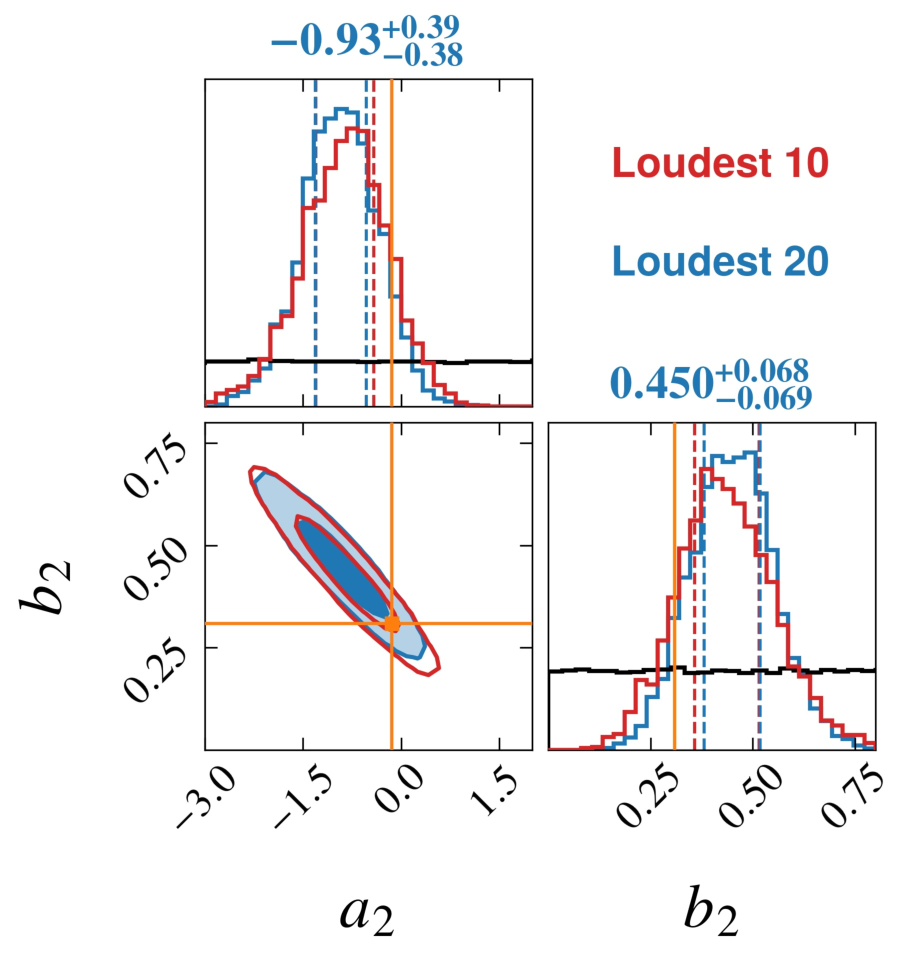
\includegraphics[width=0.5\linewidth]{comparison_corner_plot.pdf}
    \caption{Posterior distributions of the hyper parameters in the linear fitting case. 
    The contours refer to 50\% and 90\% credible regions for both inferences based on the loudest 10 and 20 events. 
    The numbers above the histograms stand for the median and the central 50\% credible interval of each marginalized distribution in the 20 event inference. 
    The orange lines represent the best fit values of the parameters in Table.~\ref{prior_table}. 
    The priors are also drawn in black for the histograms on the diagonal.}
    \label{corner2-d}
\end{figure}

\begin{figure}
\begin{minipage}[t]{0.48\textwidth}
    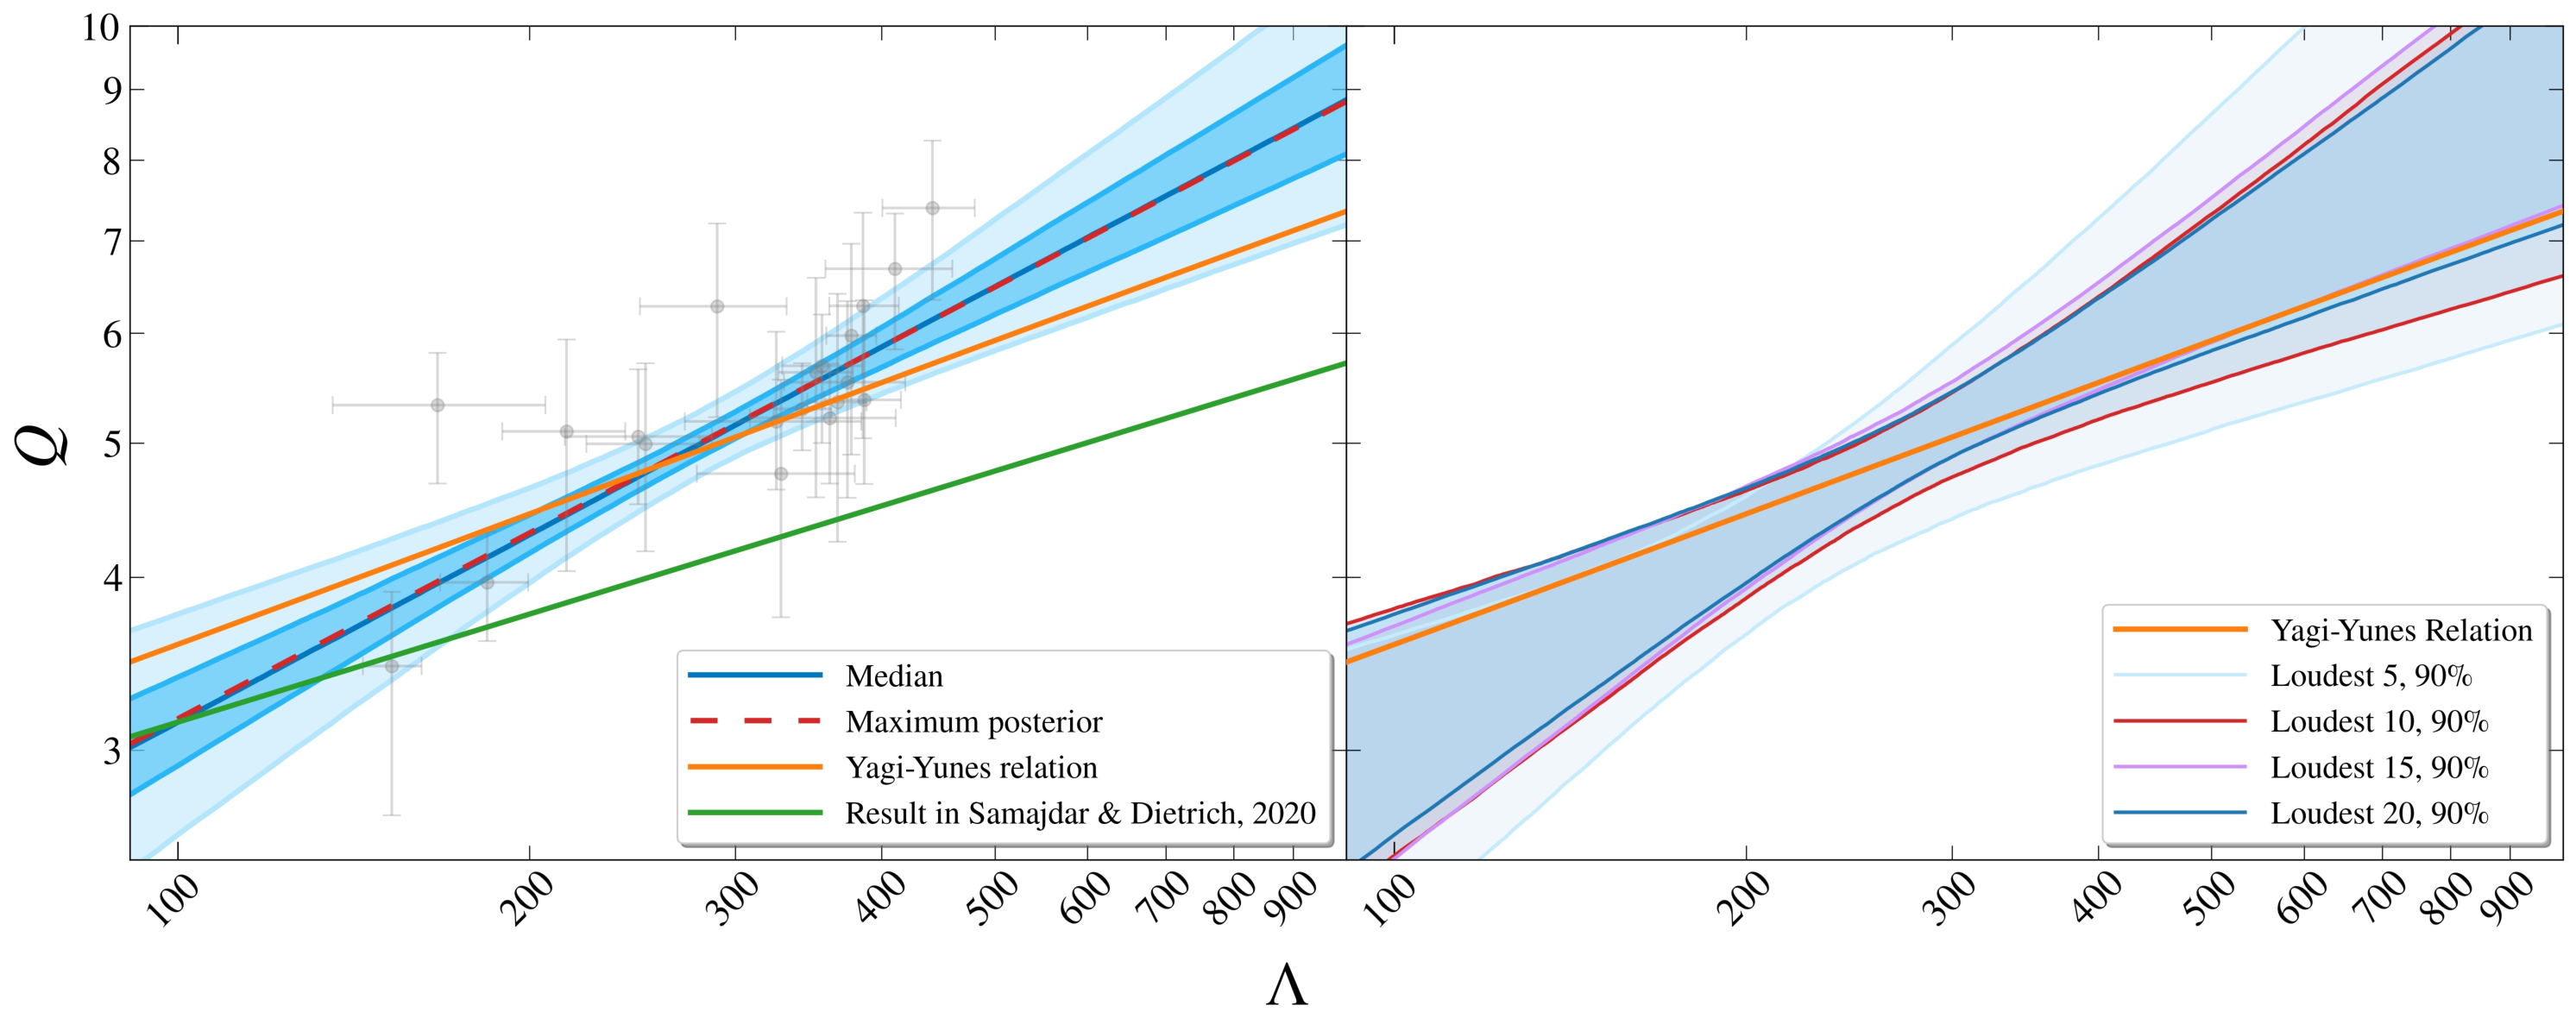
\includegraphics[width=\textwidth]{hierarchical_results_AP4_2d.pdf}
\end{minipage}
\hfill
\begin{minipage}[t]{0.48\textwidth}
    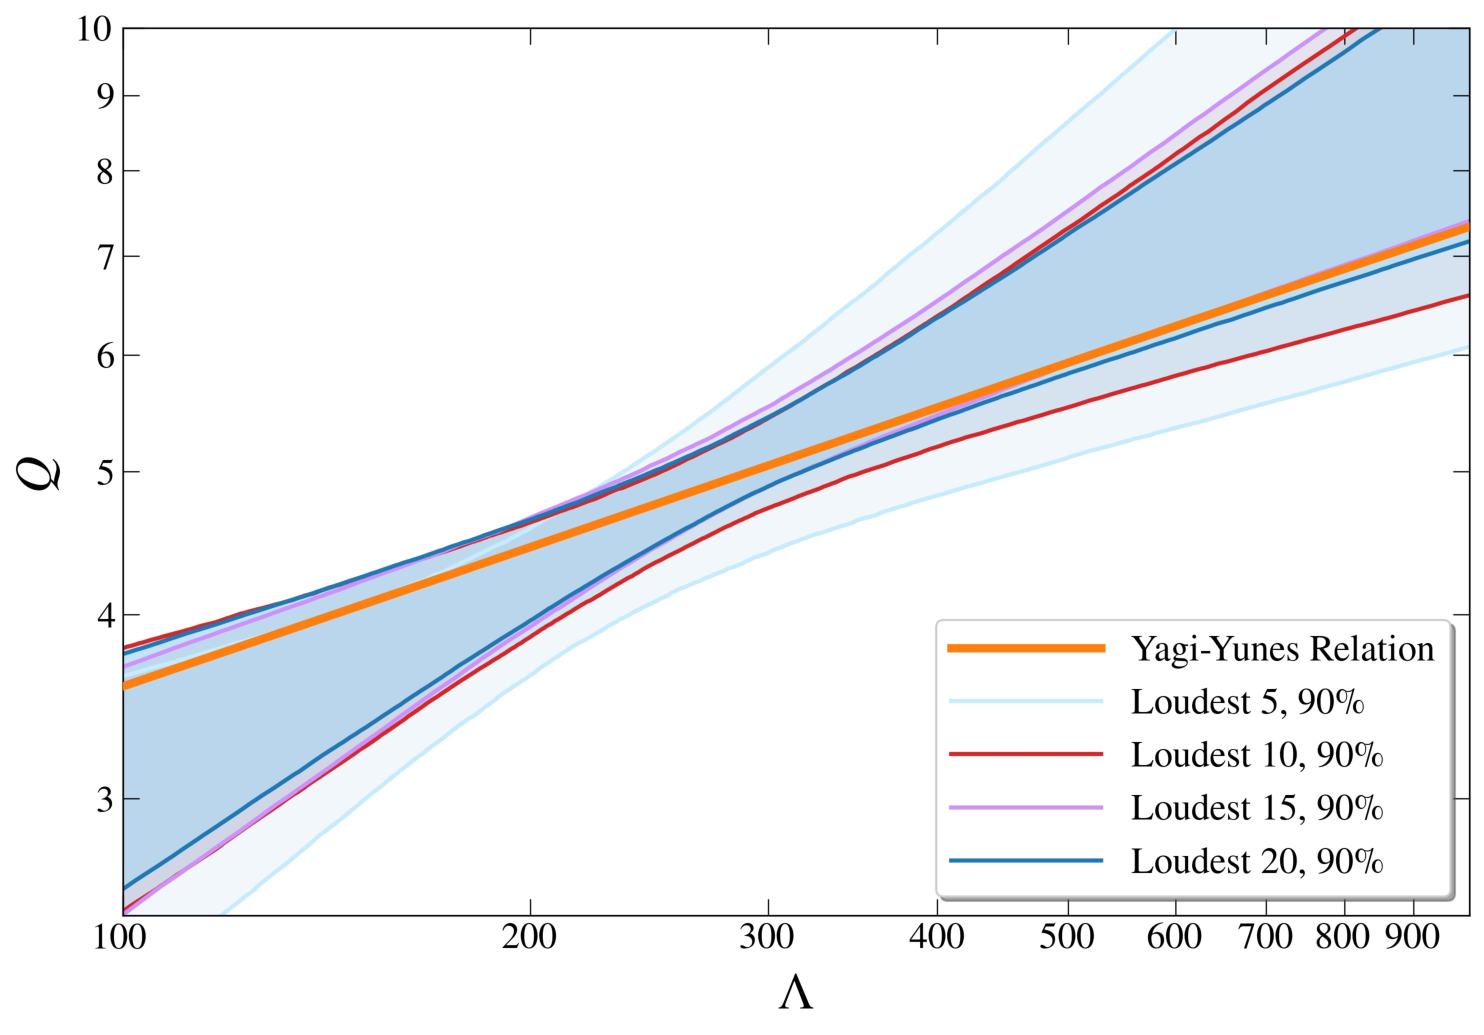
\includegraphics[width=\textwidth]{2sigma_region.pdf}
\end{minipage}
\caption{Results of the hierarchical Bayesian inference for linear Love-Q relation. 
    In the left panel, the Love-Q relation is inferred based on 20 simulated GW events. 
    The gray error bars demonstrate the $1\sigma$ credible interval of $\Lambda$ and $Q$. 
    The orange solid line represents the Yagi-Yunes Love-Q relation and the green solid line refs to the result given by Samajdar \& Dietrich, 2020~\cite{Samajdar:2020xrd}. 
    The blue regions from dark to light represent the $50\%$ and $90\%$ credible intervals of $Q$. The blue solid line and the red dashed line are the median and peak 
    of the distribution of $Q$ with certain $\Lambda$.
    Note that the Yagi-Yunes Love-Q relation is covered within the $90\%$ credible interval. 
    In the right panel, contours correspond to $90\%$ credible intervals for the inference result based on the loudest 5, 10, 15, 20 events, respectively.
    \label{2-d_Love_Q} }
\end{figure}

Based on the methods discussed above, we perform the hierarchical Bayesian inference for linear Love-Q relations. Following Ref.~\cite{Lackey:2014fwa}, 
we show how the results depend on the number of events to verify if it is valid to select sources with the highest SNR (loudest) only. 
The posterior distributions for the hyper parameters of 10 event inference and 20 event inference are both demonstrated in figure.~\ref{corner2-d} as a comparison. 
For the joint distribution in the lower left corner, we find that the credible regions of the two inferences are quite similar,
and the best fit values listed in Table.~\ref{prior_table} are close to the edge of the 50\% credible regions in the joint distribution. 
Moreover, in both cases, correlation exists between the two hyper parameters, since the credible regions are approximate oblique ellipses. 
In the diagonal corners, the peak values of the marginalized distributions for the two cases are also close to each other, indicating the dominance of events with higher SNR. 
An increase in the number of events just slightly narrows the peak width of the marginalized posteriors, and accordingly the 50\% credible region shrinks in the loudest 20 events case. 

In the left panel of figure.~\ref{2-d_Love_Q}, we plot the linear Love-Q relation according to the posterior samples. For a certain $\Lambda$, 
every sample point of hyper parameters corresponds to a $Q$ value. With $\Lambda$ fixed, we find the $50\%$ and $90\%$ credible intervals of $Q$, 
and for continuously variable $\Lambda$, the intervals combine to form a region. As we can see, the Yagi-Yunes Love-Q relation is almost covered by the $90\%$ region. 
The credible intervals are wide at both ends and narrow in the middle, as most of the events concentrate in the $\Lambda \sim 400$ region. 
In the right panel, we compare the credible regions for inferences using the loudest 5, 10, 15 and 20 events. 
The $90\%$ regions for the latter three cases almost overlap each other. This means that the loudest 10 events dominate the results, 
and thus including much quieter events will not significantly improve the results.

%=============================
\subsection{Quartic Polynomial Fitting Model}
\label{sec4_2}
%=============================

\begin{figure}
\begin{minipage}[t]{0.49\textwidth}
\centering
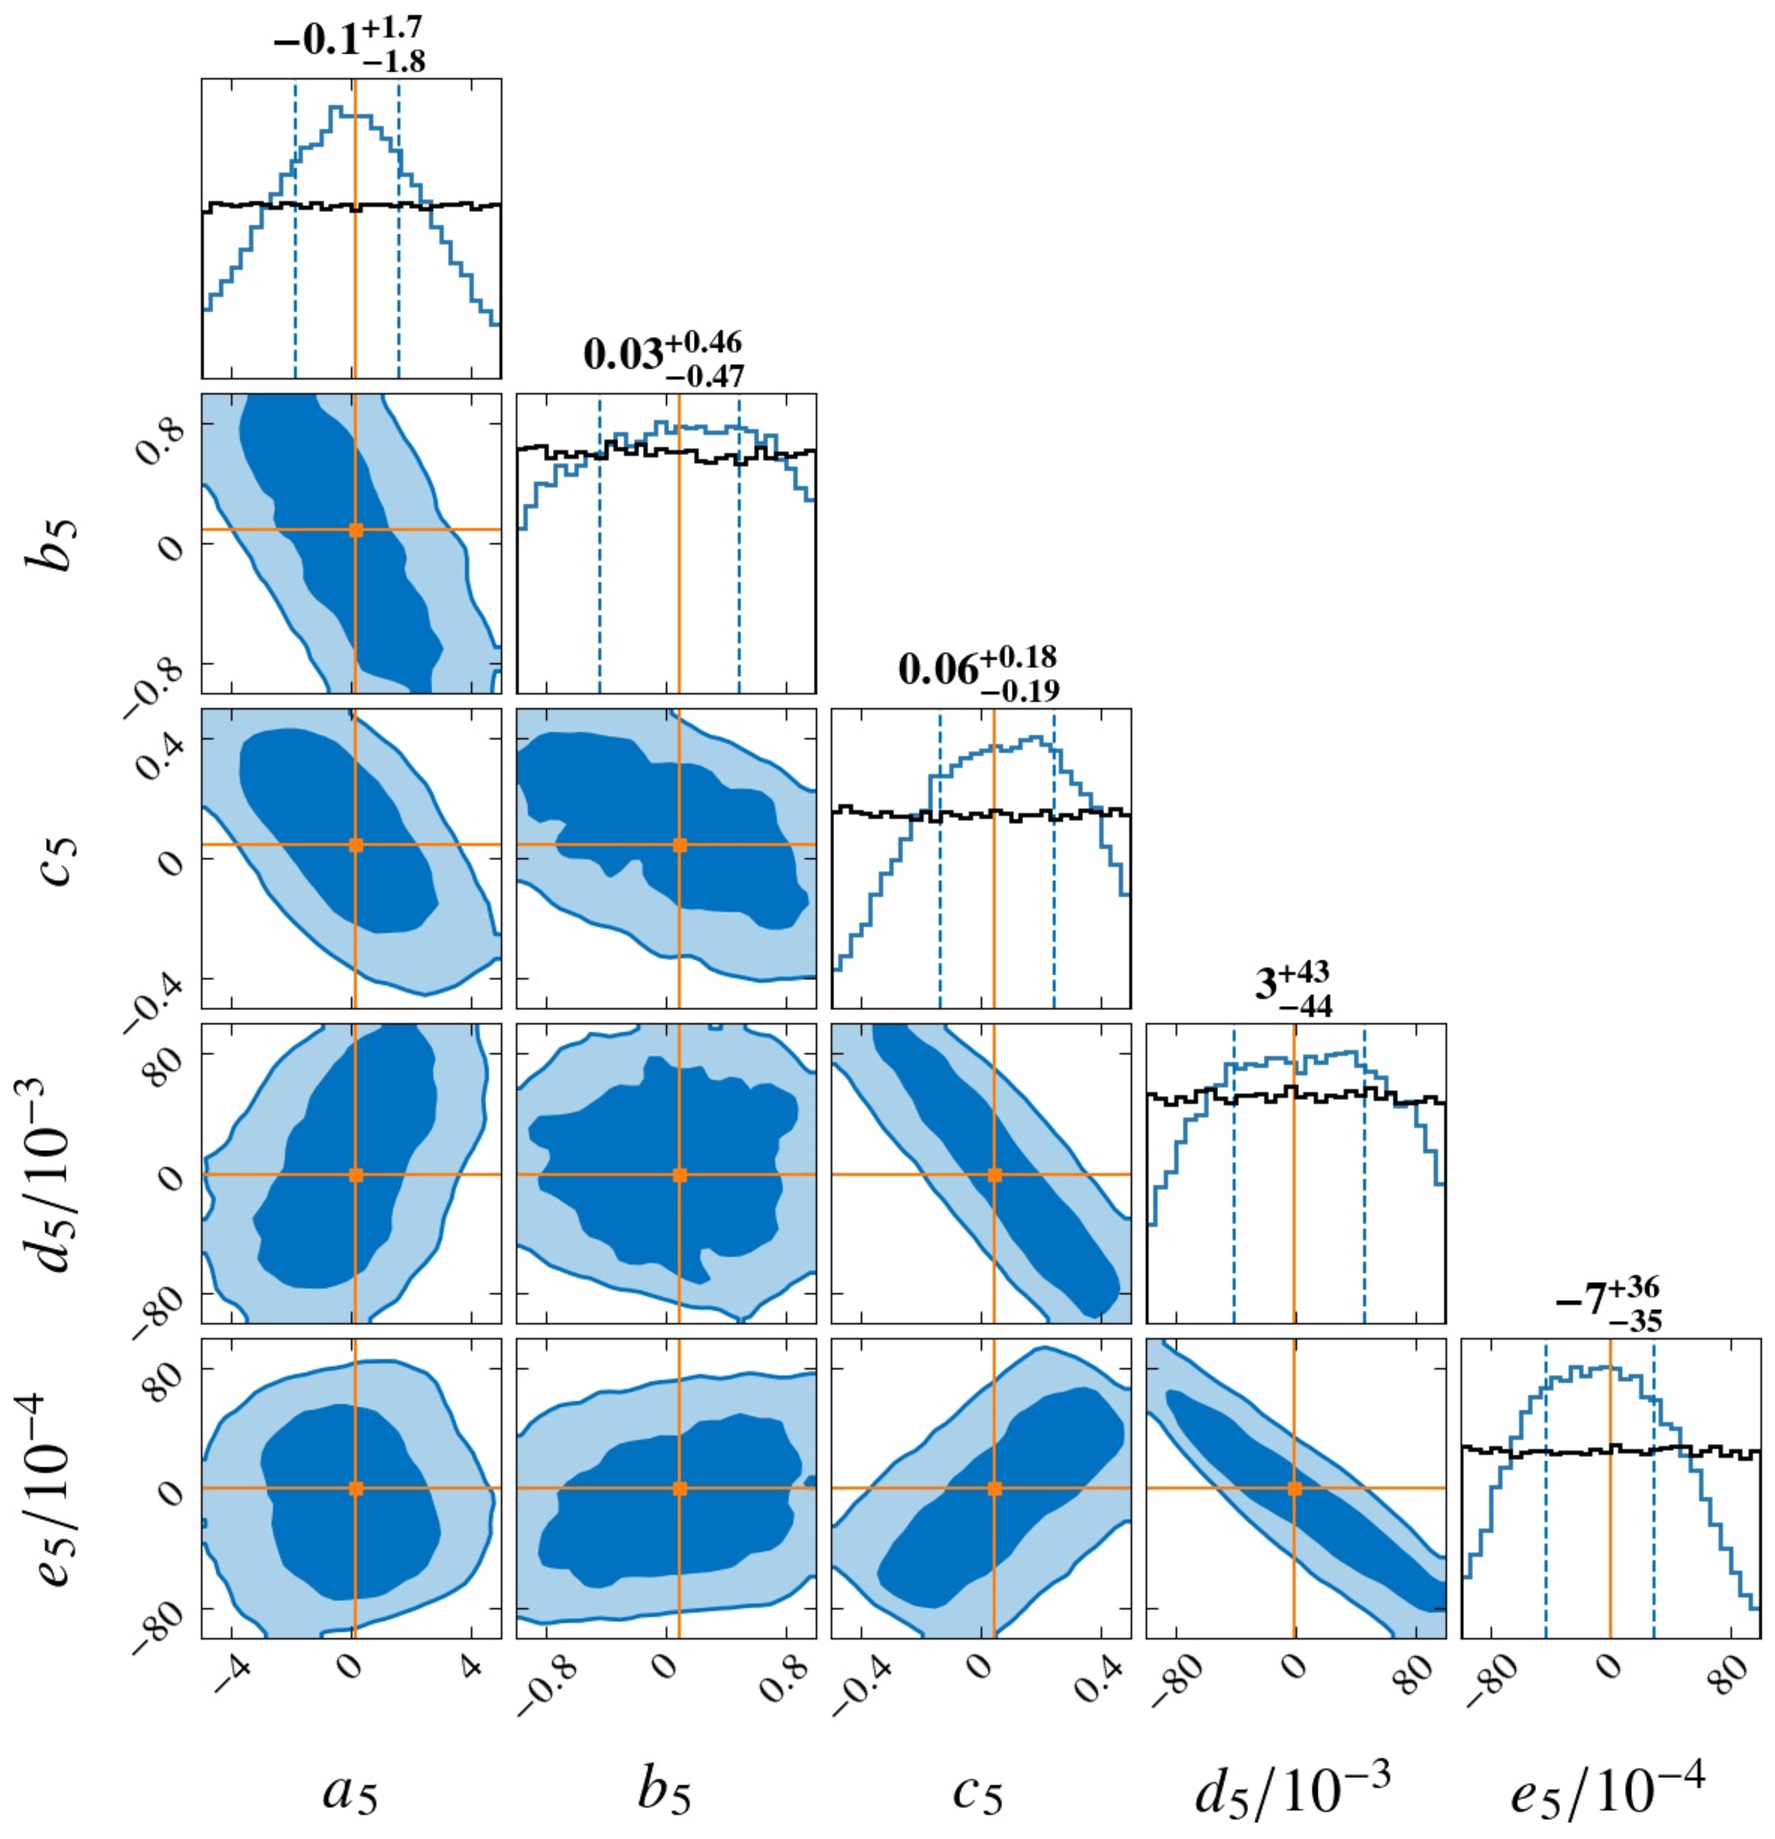
\includegraphics[width=0.8\linewidth]{Hyper_parameter_5d.pdf}% Here is how to import EPS art
\end{minipage}
\hfill
\begin{minipage}[t]{0.49\textwidth}
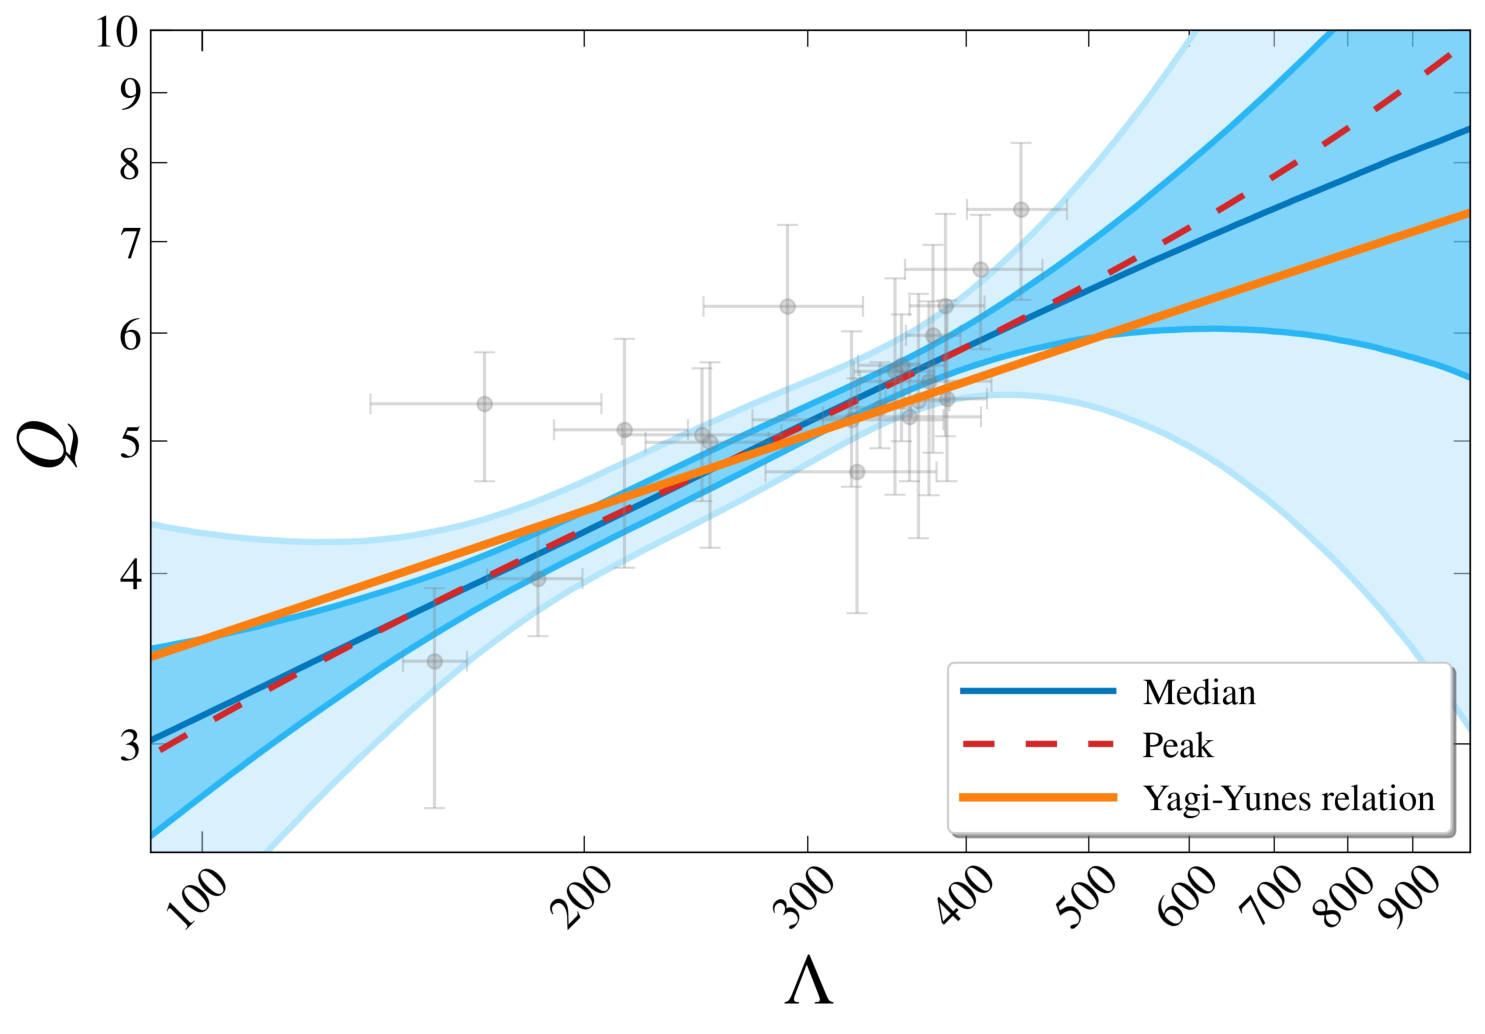
\includegraphics[width=\linewidth]{hierarchical_results_AP4_5d.pdf}
\end{minipage}
\caption{\label{5-d_Love_Q} Left panel: posterior distribution of the hyper parameters in the quartic polynomial fitting case. 
    The inference is based on all of the 20 events. The orange lines represent the values in the Yagi-Yunes Love-Q relation. 
    Right panel: similar to figure.~\ref{2-d_Love_Q}, but for the quartic polynomial fitting case. 
    Still, the Yagi-Yunes Love-Q relation is included in the $90\%$ credible region.} 
\end{figure}

For the quartic polynomial fitting model, we parameterize the Love-Q relation by eq.~(\ref{5-d_Love_Q_eq}) and perform a hierarchical Bayesian inference 
for five hyper parameter $\{a_5, b_5, c_5, d_5, e_5\}$. The left panel of figure~\ref{5-d_Love_Q} illustrates the posterior distributions of the hyper parameters for this 5-d model. 
Similarly to figure~\ref{corner2-d}, the priors and marginalized posteriors are plotted together in the diagonal histograms. 
The values taken in Yagi-Yunes Love-Q relation are closed to the marginalized distribution peaks, which become consistent with the maximum likelihood estimation given flat priors. 
Compared to the linear fitting case, these peaks are wider in the prior space and thus the credible regions in the two-parameter joint distributions become broader. 
This is reasonable since the increase in the degree of freedom makes it harder to constrain each parameter.

We summarize the 5-d Love-Q relation constraining results in the right panel of figure~\ref{5-d_Love_Q} according to the posterior distributions. We mark the $50\%$ and $90\%$ credible intervals of $Q$ 
using the same method as 2-d model. Like in figure~\ref{2-d_Love_Q} for linear Love-Q relations, the Yagi-Yunes relation almost falls within the $90\%$ region. 
In addition, the widths of the $90\%$ regions with $\Lambda \sim 400$ in figure~\ref{5-d_Love_Q} and figure~\ref{2-d_Love_Q} are close, except for the wider end in 5-d case when $\Lambda$ is large. 
This is understandable because $c_5, d_5$ and $e_5$ are much smaller than $a_5$ and $b_5$, making the $\ln^k\Lambda$ terms with $k\leq1$ dominate when $\Lambda$ is not large enough.

%=============================
\subsection{Discussion: More Fitting Models}
\label{sec4_3}
%=============================

\begin{figure}
    \begin{minipage}[t]{0.49\textwidth}
    \centering
    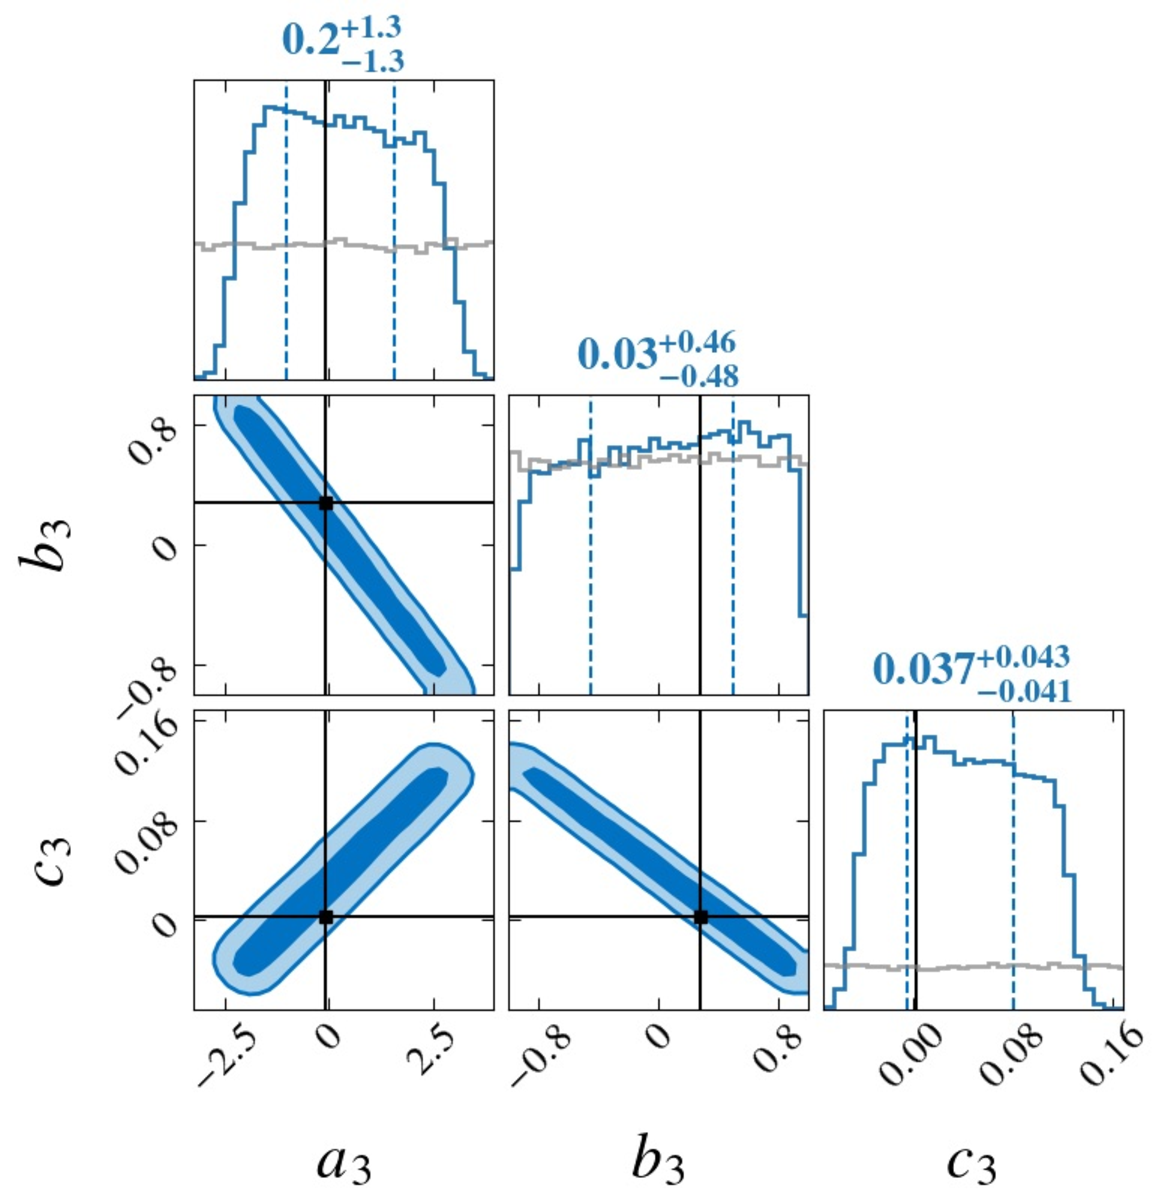
\includegraphics[width=0.8\linewidth]{Hyper_parameter_3d.pdf}% Here is how to import EPS art
    \end{minipage}
    \hfill
    \begin{minipage}[t]{0.49\textwidth}
    \centering
    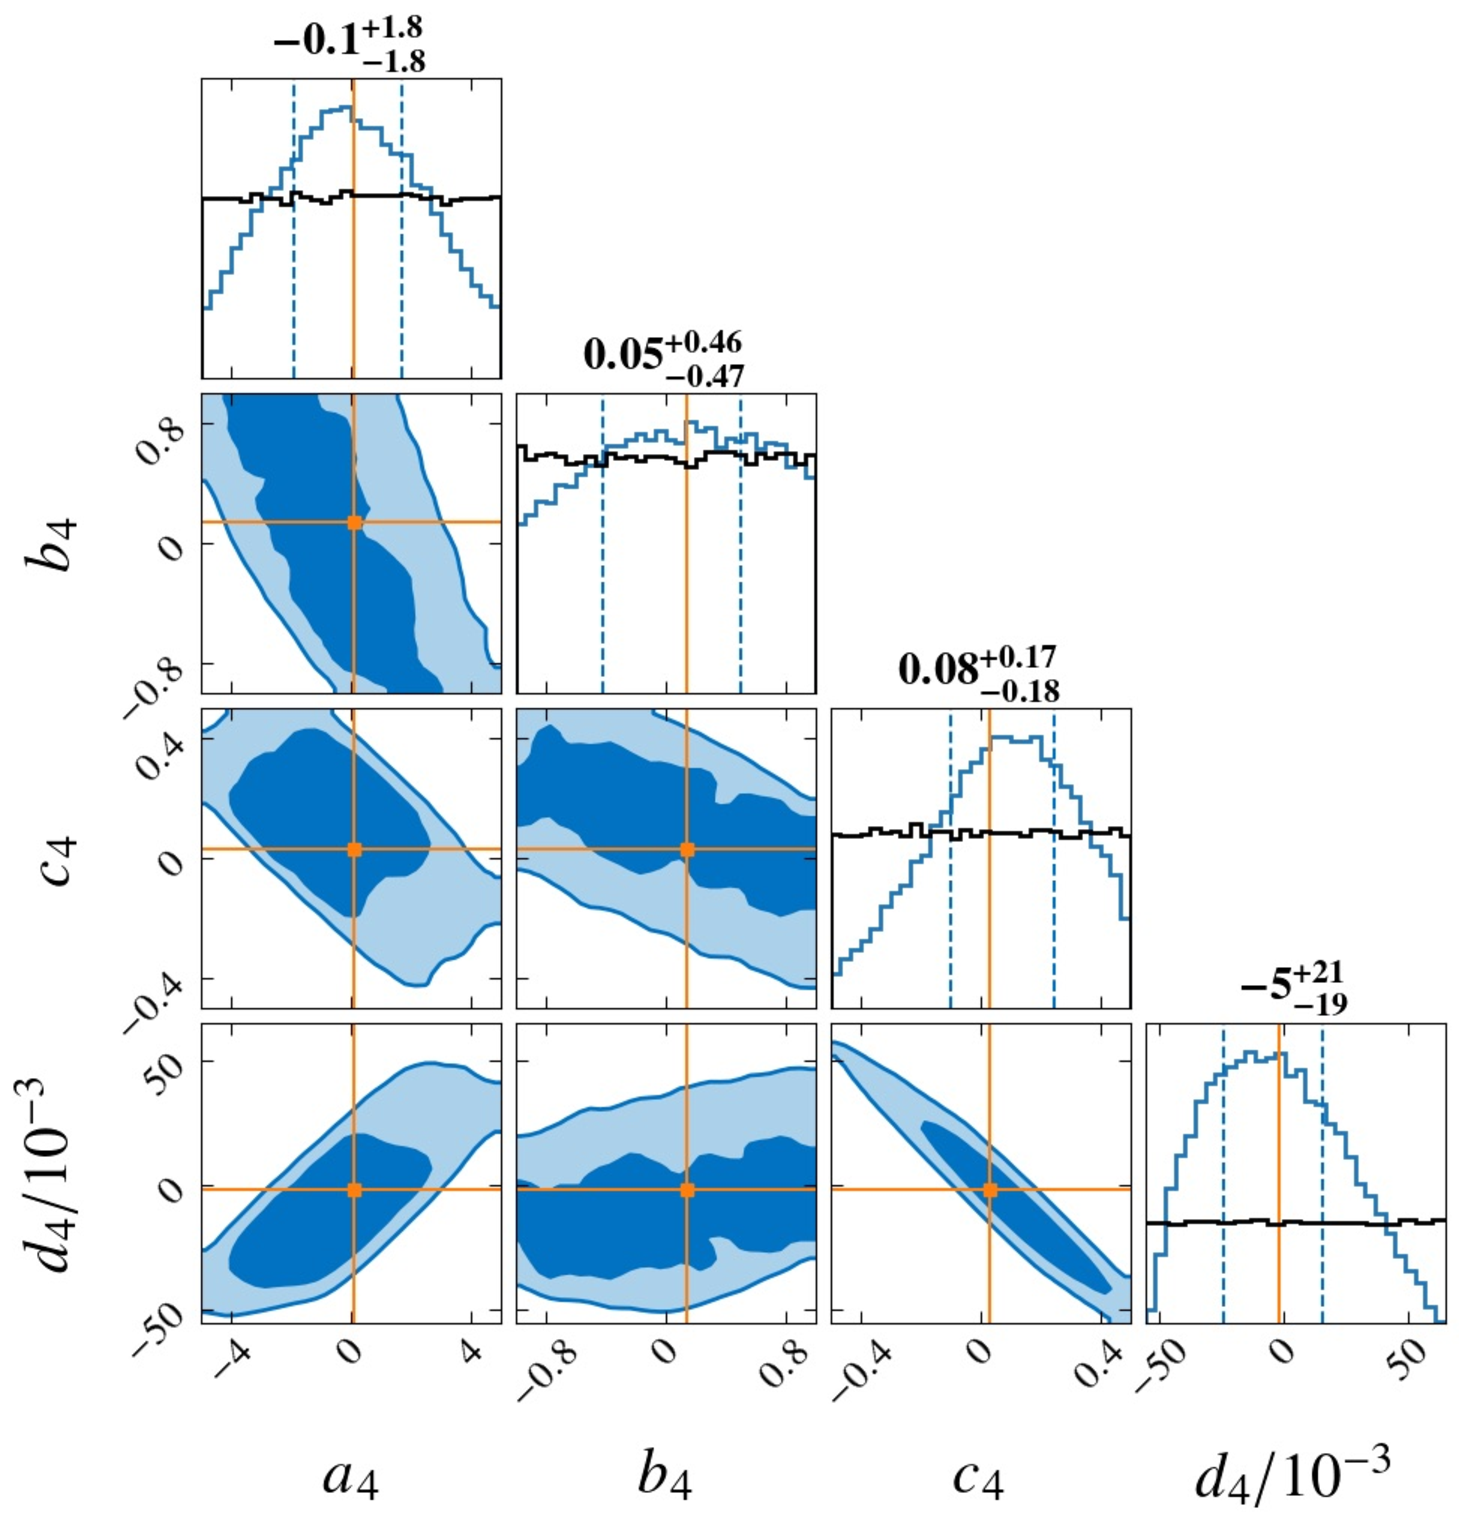
\includegraphics[width=0.8\linewidth]{Hyper_parameter_4d.pdf}
    \end{minipage}
    \vspace{3mm}
    \begin{minipage}[t]{0.49\textwidth}
    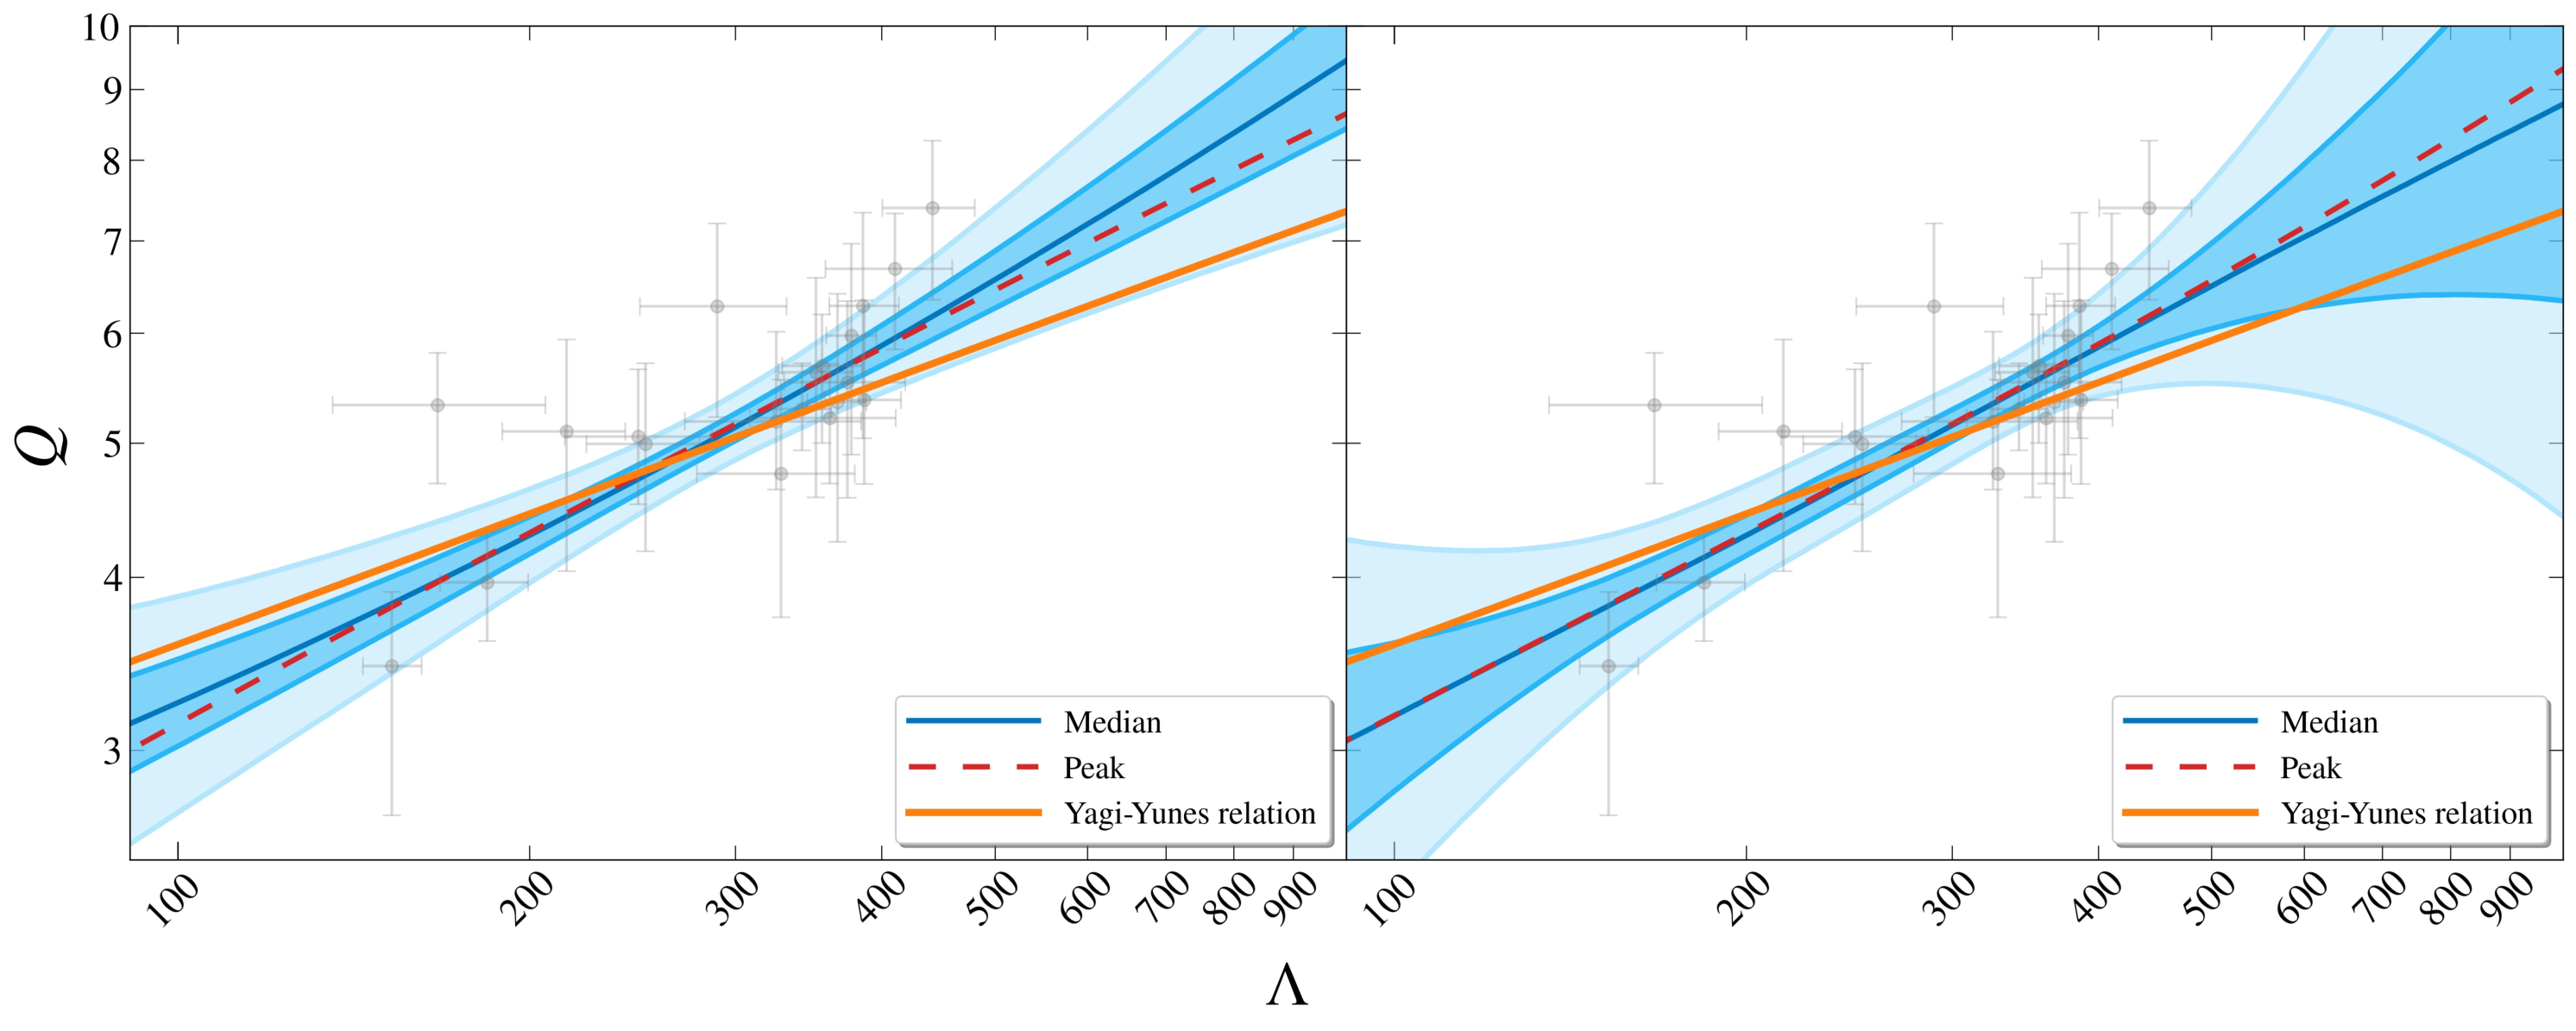
\includegraphics[width=\linewidth]{hierarchical_results_AP4_3d.pdf}% Here is how to import EPS art
    \end{minipage}
    \hfill
    \begin{minipage}[t]{0.49\textwidth}
    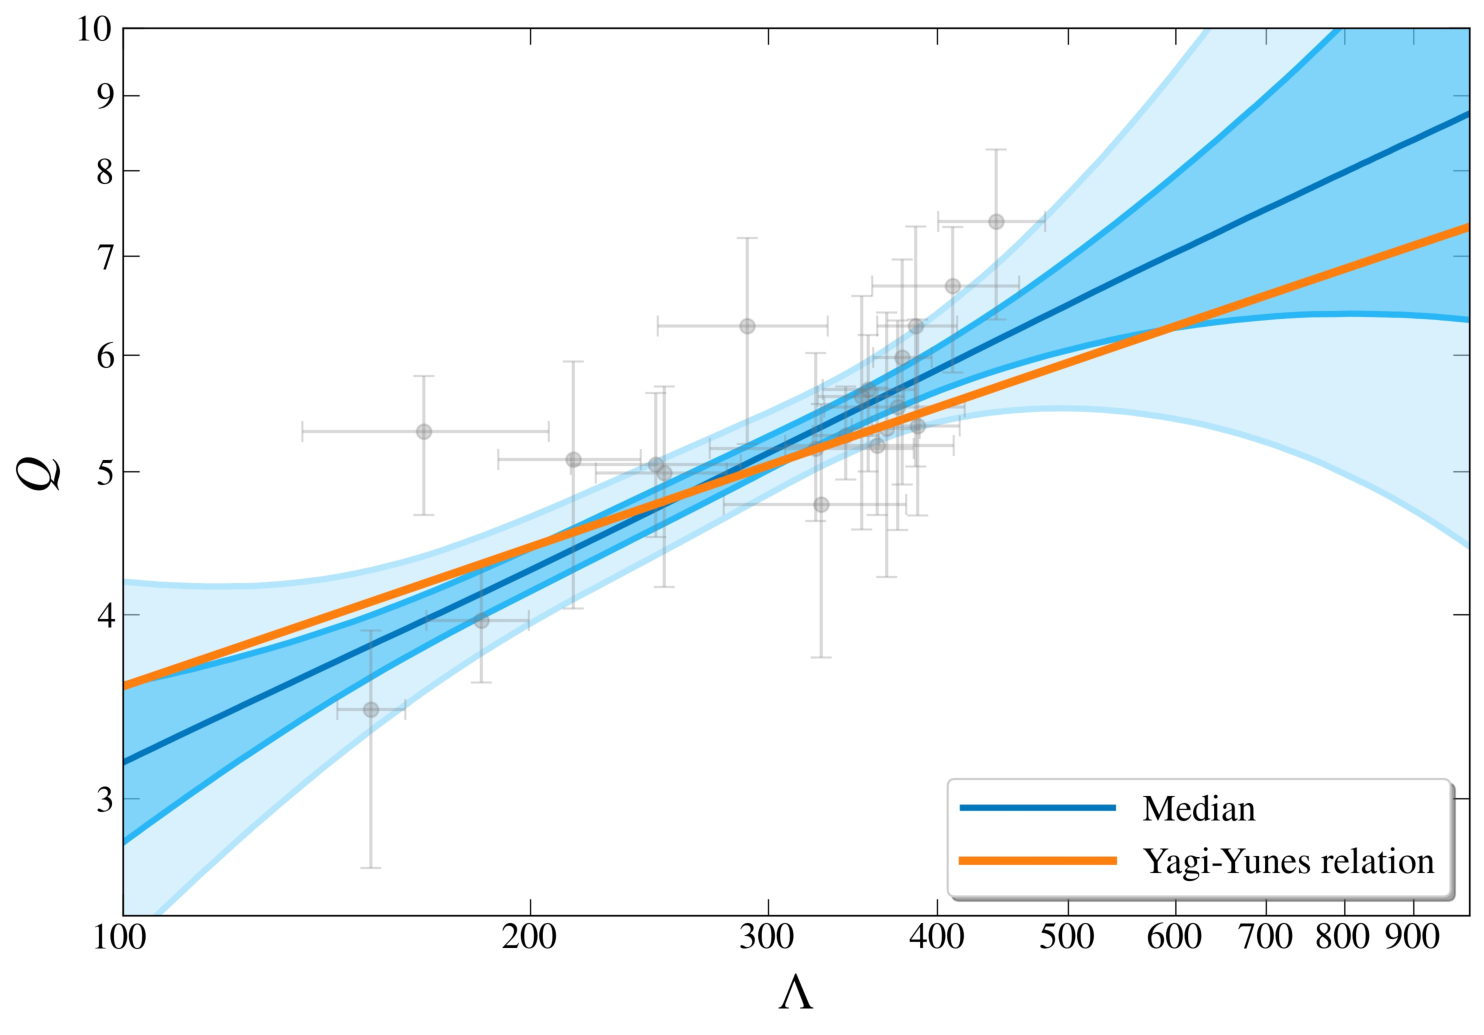
\includegraphics[width=\linewidth]{hierarchical_results_AP4_4d.pdf}
    \end{minipage}
    \caption{\label{3-d_4-d_Love_Q} Results of quadratic and cubic polynomial (3-d and 4-d) fitting models. The 
    two upper panels demonstrate the posteriors of the hyper parameters. And the best fit values (see table~\ref{prior_table}) 
    are marked in orange. The two bottom panels present the inference results in Love-Q plane, similar to 
    figure~\ref{2-d_Love_Q}.
    }
\end{figure}

We have mentioned in section~\ref{sec4_2} that it will be harder to constrain every hyper parameter as the 
degree of freedom increases, thus we perform hyper parameter inferences for quadratic and cubic polynomial, 
i.e. 3-d and 4-d, fitting models. Figure~\ref{3-d_4-d_Love_Q} demonstrates the posteriors and the corresponding 
Love-Q inference results for 3-d and 4-d models. In the 3-d case, we find strong degeneracy among the three parameters. 
The marginalized posterior distributions of $a_3$ and $c_3$ have very wide and flat peaks, while $b_3$ is so poorly 
constrained that its posterior is similar to its prior. When it comes to the 4-d inference results, degeneracy still 
emerges and again we find the marginalized posterior of one hyper parameter $b_4$ resemble the prior. These results 
imply that for our simulation data size, a 2-d linear fitting model is enough and the two fitting coefficients can be 
well constrained by our hierarchical Bayesian inference.

Same as before, we plot the constraint of Love-Q relation according to the posterior samples in the two lower panels 
of figure~\ref{3-d_4-d_Love_Q}. Like 2-d and 5-d results, the width of the $90\%$ region where most of the data points 
gather is insensitive to our parameterization of the Love-Q relation. We expect a better constraint to the both ends of 
the 90\% regions based on more GW events, which may contain more information for the behavior of the Love-Q relation 
with $\Lambda \sim 100$ or $\Lambda > 500$.

%=============================
\section{Testing Modified Gravity: Dynamical Chern-Simons Gravity}
\label{sec5}
%=============================

\begin{figure}[htbp]
    \centering
    \begin{minipage}{0.48\linewidth}
        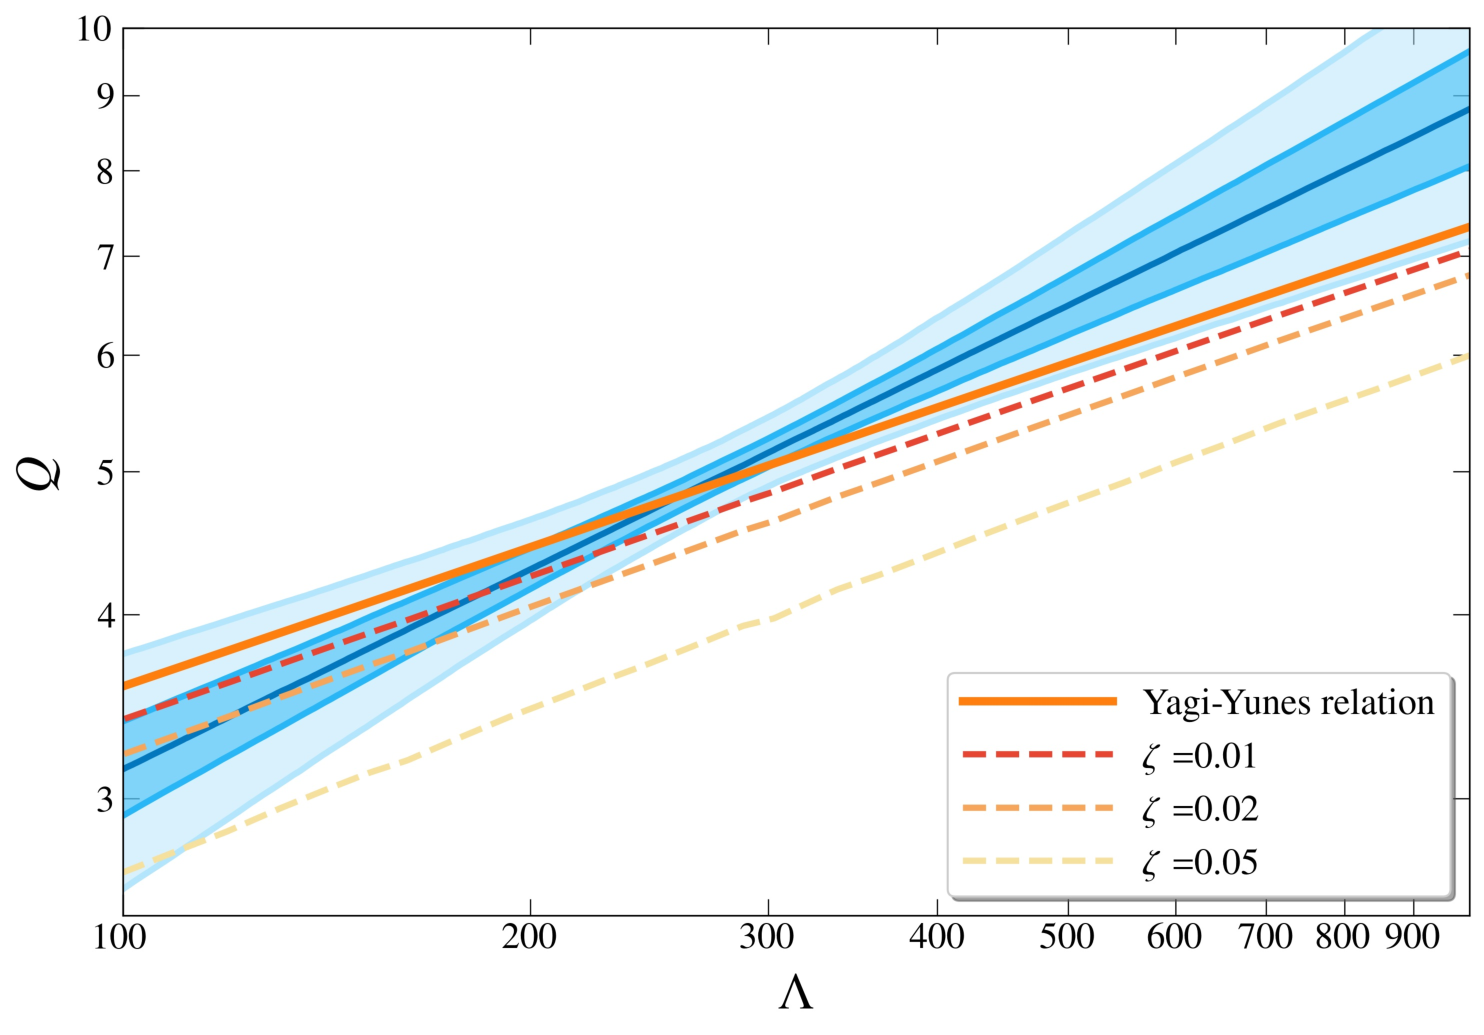
\includegraphics[width=\linewidth]{CS_zeta_AP4_2d.pdf}
    \end{minipage}
    \hfill
    \begin{minipage}{0.48\linewidth}
        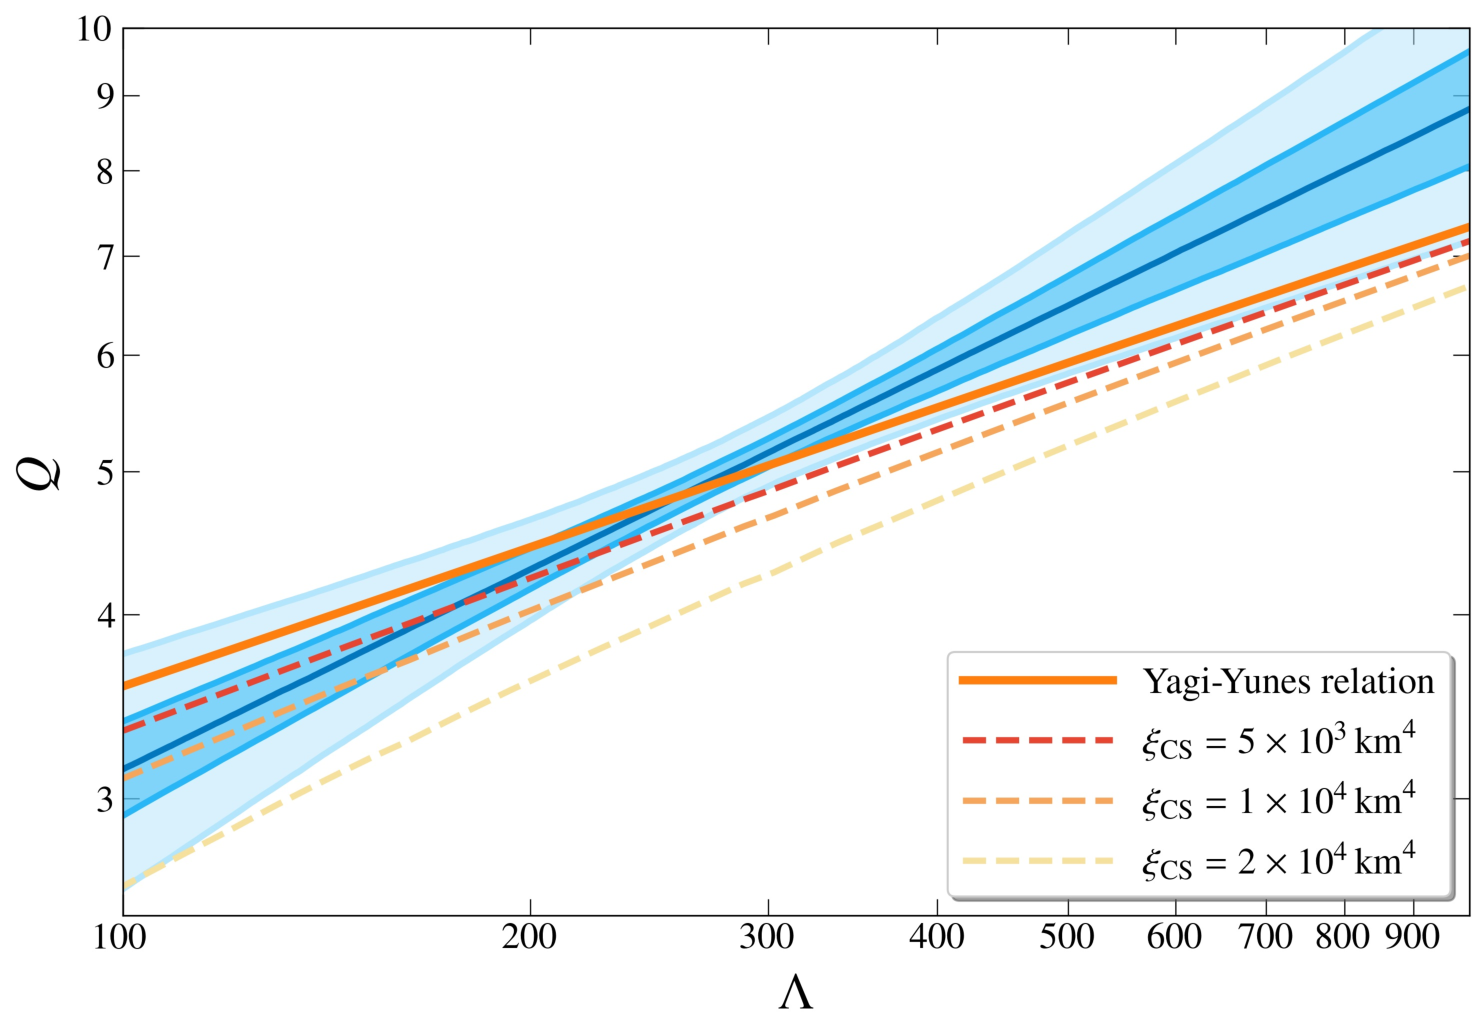
\includegraphics[width=\linewidth]{CS_xi_cs_AP4_2d.pdf}
    \end{minipage}
    \vspace{3mm}
    \begin{minipage}{0.48\linewidth}
        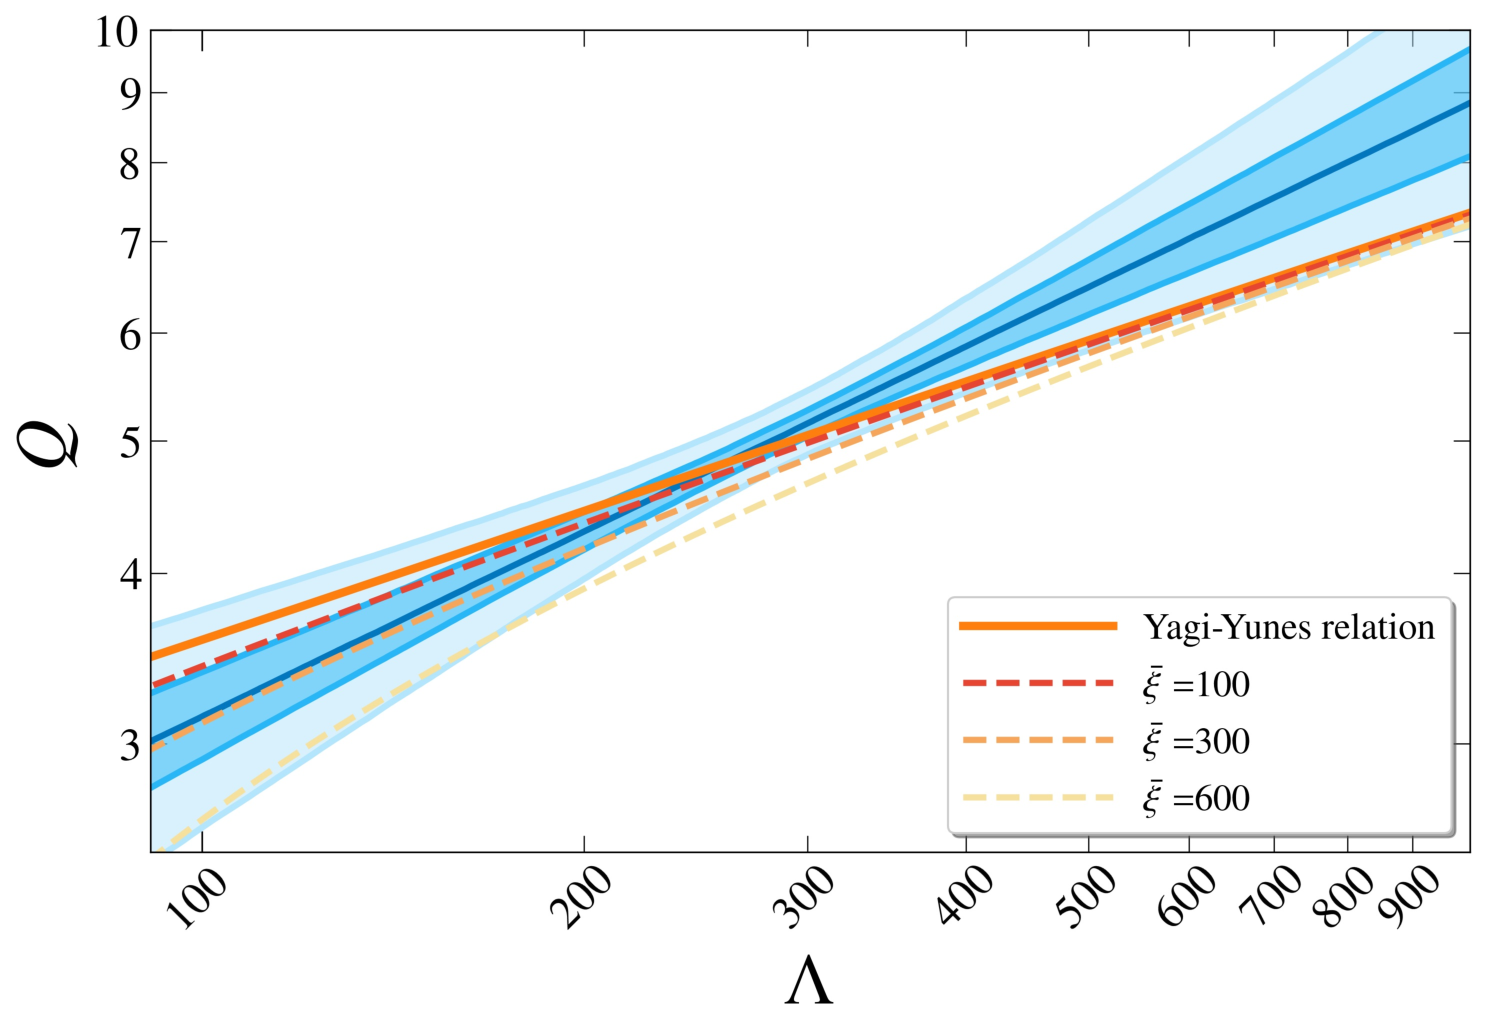
\includegraphics[width=\linewidth]{CS_xi_bar_AP4_2d.pdf}
    \end{minipage}
    \caption{Comparison of the hierarchical inference results and CS predictions with different coupling constants fixed. 
    The blue regions are the same as figure~\ref{2-d_Love_Q} (Linear fitting model). For each of the coupling constants of CS gravity 
    $\zeta, \xi_{\mathrm{CS}}$ and $\bar\xi$, three possible values are taken and the corresponding Love-Q relations 
    for AP4 EOS are drawn respectively as references.}
    \label{cs_Love_Q}
\end{figure}

For some parity-violating modified gravity theories that have not been 
stringently constrained yet, a I-Love-Q test can be powerful due to the significant difference in I-Love-Q relation emerging in these theories~\cite{Yagi_2017, Yunes:2025xwp}. 
We select the dynamical Chern-Simons (dCS) gravity~\cite{Jackiw:2003pm, Smith:2007jm, Alexander:2009tp} for discussion, considering that the I-Love-Q relation degeneracy only occurs in the limit 
when the coupling constant becomes infinitesimal~\cite{Yagi:2013bca, Yagi:2013awa, Gupta:2017vsl}.
By comparing the uncertainty given by our inference results with the deviation originating from the dCS gravity, we can see to what extent 
can our results constrain the coupling constants in dCS gravity at most.

The dCS gravity introduces parity violation and quadratic curvature terms into the action~\cite{Alexander:2009tp, Gupta:2017vsl}
\begin{equation}
    \label{cs_action}
    S = \int \mathrm{d}^4 x \sqrt{-g}\left[ \kappa_g \mathcal{R} + \frac{\alpha}{4} \mathcal{\vartheta} \mathcal{R}_{\nu\mu\rho\sigma} {}^{*}\mathcal{R}^{\mu\nu\rho\sigma} - \frac{\beta}{2}(\nabla_{\mu}\mathcal{\vartheta}\nabla^{\mu}\mathcal{\vartheta}+2V(\mathcal{\vartheta})) + \mathcal{L}_{\mathrm{mat}}\right]\,,
\end{equation}
where $\mathcal{R}$ is the Ricci scalar, $\mathcal{L}_{\mathrm{mat}}$ is the matter Lagrangian density, $g$ is the determinant of the metric, $\kappa_g\equiv 1/(16\pi)$, and $\alpha$ and $\beta$ 
are the coupling constants in dCS gravity. We assume that the pseudo-scalar field $\mathcal{\vartheta}$ is dimensionless, thus the quantity $\xi_{\mathrm{CS}}^{1/4} \equiv [\alpha^2/(\kappa\beta)]^{1/4}$ \
can be regarded as a characteristic length scale of the theory. Current Solar System observations have constrained $\xi_{\mathrm{CS}}^{1/4}< \mathcal{O}(10^8)$km~\cite{Ali-Haimoud:2011zme, Yagi:2012ya}. 

For our Love-Q test, ref.~\cite{Yagi:2013mbt} obtained the dCS correction to the NS quadrupole moment and ref.~\cite{Yagi:2011xp} indicates 
that the tidal deformability is the same as in GR at leading order in small coupling approximation $\zeta \equiv \xi_{\mathrm{CS}} M^2/R^6 \ll 1$, 
regarding the dCS gravity as an effective theory. Refs.~\cite{Yagi_2017, Yagi:2013mbt} have discussed the I-Love-Q relations under dCS gravity 
and find that the relations remain universal when we normalize the variables with respect to $\bar{\xi}\equiv \xi_{\mathrm{CS}}/M^4$, 
while become EOS-sensative with $\xi_{\mathrm{CS}}$ or $\zeta$ fixed. 

Following ref.~\cite{Yagi_2017}, we calculate the dCS Love-Q relation with $\zeta, \xi_{\mathrm{CS}}$ and $\bar{\xi}$ fixed respectively 
for the AP4 EOS, which has been assumed in our simulation in section~\ref{sec3}. The results are demonstrated in figure~\ref{cs_Love_Q}. 
We compare the hierarchical Bayesian inference constraint of the Love-Q relation using linear fitting model (figure~\ref{2-d_Love_Q}) with 
some possible Love-Q relations with respect to certain coupling constants in dCS gravity. From figure~\ref{cs_Love_Q} we can conclude that 
our Love-Q test of dCS gravity can constrain the characteristic length $\xi_{\mathrm{CS}}^{1/4} < \mathcal{O}(10^2)$km, which is in agreement  
with the results given by refs.~\cite{Yagi:2013bca, Yagi:2013awa}.

%=============================
\section{Conclusion}
\label{sec6}
%=============================

This work has constructed a hierarchical Bayesian framework to estimate the Love-Q relation of NSs. By separating the single-event inferences and 
hyper parameter inference, this framework manifests high computational efficiency and provides a sophisticated statistical 
method for hyper parameter estimation. We applied this framework to simulated GW events for a next-generation detector network 
to examine the potential of constraining the Love-Q relation with GW observations. The results demonstrated that with the next-generation GW detector network, 
one can obtain a reliable measurement of the Love-Q relation through hierarchical Bayesian inference. We have also verified that the inference results of the 
hyper parameters are dominated by events with the highest SNRs, which is consistent with the findings of ref.~\cite{Lackey:2014fwa}.

We then investigated the impact of different parameterizations for Love-Q relation on the inference. 
We found that constraint of the Love-Q relation is insensitive to the parameterization in the region where most data points gather.
Also, as shown by the posterior distributions, degeneracies between hyper parameters exist in all cases studied. 
Furthermore, for all but the linear model, at least one hyper parameter was poorly constrained, exhibiting wide and flat posterior. 
These results indicate that a two-parameter (linear) model is sufficient for our data volume (20 GW events).

Finally, as a practical application, we compared our inference results with the theoretical predictions of the dCS gravity. The Love-Q relation measurement precision 
of our hierarchical Bayesian inference allows us to place a constraint on the dCS characteristic length $\xi_{\mathrm{CS}}^{1/4} < \mathcal{O}(10^2)$km. 
This result is consistent with previous works~\cite{Yagi:2013bca, Yagi:2013awa} and highlights the power of the Love-Q relation inference for testing gravity theories.

%=============================
\acknowledgments

\clearpage

\bibliographystyle{JHEP}
% \bibliographystyle{unsrt}
\bibliography{HBAGW_jcap}
\end{document}
